% arara: pdflatex
% arara: bibtex
% arara: bibtex
% arara: pdflatex
% arara: pdflatex

\documentclass{dcthesis}

%This version of the thesis template has been updated for the February 2017 thesis guidelines provided by the School of Graduate and Advanced Studies by David Freund and Daryl DeFord.

%  Some good options are draft and singlespacing, for drafts, and *final*,
%for the final cut, and noheadings, for a printout without headings.  
%You can also use the copyright option to add a copyright.  Note:
%final will enforce a bunch of different options, like oneside, 12pt
%and doublespacing, as well as make the margins correct.   Draft, has
%larger margins and is appropriate for two sided printing.   


%%%%%%%%%%%%%%%%%%%%%%%%%%%
%%%%    IMPORTANT     %%%%%
%%%%%%%%%%%%%%%%%%%%%%%%%%%
%
%  Because dvips doesn't know/care about the page size of the dvi file
%  its working on, and because its so important that the margins of
%  your thesis are correct you have to make sure that you are using
%  the command dvi -t letter *thesisnamehere*
%
%  If you are using a terminal this is straightforward, but if you are
%  using a tex editing program it make take a little bit of searching
%  before you figure out how to make this work. 
%  
%  Alternatively, you might consider compiling using pdflatex, which
%  compiles straight to a PDF and doesn't have this problem.  

%%%%%%%%%%%%%%%%%%%%%%%%%%%%%%%%%%%%%%%%%%%%%%%%%%
% Some Defaults
%%%%%%%%%%%%%%%%%%%%%%%%%%%%%%%%%%%%%%%%%%%%%%%%%%
\committee[F. Jon Kull, Ph.D.]{}{}{}{}
\school{Dartmouth College}{Hanover, New Hampshire}
\degree{Doctor of Philosophy}
\field{Mathematics}

%%%%%%%%%%%%%%%%%%%%%%%%%%%%%%%%%%%%%%%%%%%%%%%%%%
% Additional Packages (add as desired)
%%%%%%%%%%%%%%%%%%%%%%%%%%%%%%%%%%%%%%%%%%%%%%%%%%
\usepackage{amsmath,amssymb,amsthm,amsxtra}
\usepackage{mathrsfs} 
\usepackage{lipsum}
\usepackage{xcolor}
\usepackage{hyperref}
\hypersetup{colorlinks=true,urlcolor=blue,citecolor=blue,linkcolor=blue}
\usepackage{tikz}
\usepackage{colonequals}
\usetikzlibrary{arrows,calc,automata,shadows,backgrounds,positioning,intersections,fadings,decorations.pathreplacing,shapes,snakes, matrix}
\usepackage{tikz-cd}
\tikzset{commutative diagrams/.cd, arrow style = tikz, diagrams = {>=latex}}
\tikzset{>=latex}

%\usepackage{index} %Uncomment if you would like to have an index. Compiling with an index takes more work than compiling without one. You will have to look up how to use the index package.

%%%%%%%%%%%%%%%%%%%%%%%%%%%%%%%%%%%%%%%%%%%%%%%%%%
%Formatting
%%%%%%%%%%%%%%%%%%%%%%%%%%%%%%%%%%%%%%%%%%%%%%%%%%
%  Change or add to as desired. 
%  These two commands make the first enumerations look like (a)
%  And the second level like (i).  
% \renewcommand{\labelenumi}{(\alph{enumi})}
% \renewcommand{\labelenumii}{(\roman{enumii})}
%  These commands make the section headings Boldface and not all
%  caps. It also removes the chapter numbers  
\renewcommand{\chaptermark}[1]{\markboth{{\sc #1}}{{\sc #1}}}
\renewcommand{\sectionmark}[1]{\markright{{\sc \thesection\ #1}}}
%  These commands have lowercase headings with chapter numbers. 
%\renewcommand{\chaptermark}[1]{markboth{#1}{}}
%\renewcommand{\sectionmark}[1]{\markright{\thesection\ #1}} 
\newcommand{\PP}{\mathbb P}
\newcommand{\CC}{\mathbb C}
\newcommand{\QQ}{\mathbb Q}
\newcommand{\ZZ}{\mathbb Z}
\renewcommand{\AA}{\mathbb A}
\newcommand{\defi}[1]{\textsf{#1}}
\newcommand{\jv}[1]{{\color{red} \sf JV: [#1]}}
\newcommand{\mm}[1]{{\color{blue} \sf MM: [#1]}}
\newcommand{\wt}[1]{\widetilde{#1}}
\newcommand{\QQal}{{\mathbb Q}^{\textup{al}}}
\newcommand{\QQab}{{\mathbb Q}^{\textup{ab}}}
\newcommand{\QQbar}{{\mathbb Q}^{\textup{al}}}
\newcommand{\Kal}{{{K}^{\textup{al}}}}
\newcommand{\Kab}{{K}^{\textup{ab}}}
\newcommand{\kbar}{\overline{k}}
\newcommand{\Kbar}{\overline{K}}
\newcommand{\LL}{\mathscr L}
\newcommand{\sm}{\setminus}

\DeclareMathOperator{\Div}{Div}
\DeclareMathOperator{\Pic}{Pic}
\DeclareMathOperator{\ddiv}{div}
\DeclareMathOperator{\sat}{sat}
\DeclareMathOperator{\ddeg}{deg}
\DeclareMathOperator{\ddim}{dim}
\DeclareMathOperator{\rred}{red}
% \renewcommand{\rred}{\operatorname{red}}
\DeclareMathOperator{\Lifts}{Lifts}
\DeclareMathOperator{\order}{order}
\DeclareMathOperator{\Aut}{Aut}
\DeclareMathOperator{\PGL}{PGL}
\DeclareMathOperator{\Mon}{Mon}
\DeclareMathOperator{\Gal}{Gal}
\DeclareMathOperator{\supp}{supp}
\DeclareMathOperator{\ord}{ord}
\DeclareMathOperator{\mult}{mult}
\DeclareMathOperator{\stab}{stab}
\DeclareMathOperator{\orb}{orb}

%%%%%%%%%%%%%%%%%%%%%%%%%%%%%%%%%%%%%%%%%%%%%%%%%%
% Theorem Declarations
%%%%%%%%%%%%%%%%%%%%%%%%%%%%%%%%%%%%%%%%%%%%%%%%%%
% A basic set of theorem declarations.  Add or remove as desired. 
% \newtheorem{prop}{Proposition}[chapter]
\newtheorem{prop}{Proposition}[section]
\newtheorem{theorem}[prop]{Theorem}
\newtheorem{conj}[prop]{Conjecture}
\newtheorem{lemma}[prop]{Lemma}
\newtheorem{corr}[prop]{Corollary}
\theoremstyle{definition}
\newtheorem{definition}[prop]{Definition}
\newtheorem{alg}[prop]{Algorithm}
\newtheorem{notation}[prop]{Notation}
\theoremstyle{remark}
\newtheorem{remark}[prop]{Remark}
\newtheorem{example}[prop]{Example}
\newtheorem*{claim}{Claim}
% numberwithin section for equations and figures
\numberwithin{equation}{section}
\numberwithin{figure}{section}
% \renewcommand{\thefigure}{\arabic{figure}}

%%%%%%%%%%%%%%%%%%%%%%%%%%%%%%%%%%%%%%%%%%%%%%%%%%
%Indices
%%%%%%%%%%%%%%%%%%%%%%%%%%%%%%%%%%%%%%%%%%%%%%%%%%
%This is for an index.  More work is needed for a notation index
%\makeindex

%%%%%%%%%%%%%%%%%%%%%%%%%%%%%%%%%%%%%%%%%%%%%%%%%%
% Macros
%%%%%%%%%%%%%%%%%%%%%%%%%%%%%%%%%%%%%%%%%%%%%%%%%%
% Add your math macros here

%%%%%%%%%%%%%%%%%%%%%%%%%%%%%%%%%%%%%%%%%%%%%%%%%%
% Title Page Information
%%%%%%%%%%%%%%%%%%%%%%%%%%%%%%%%%%%%%%%%%%%%%%%%%%
%  Your personal info goes here!
\title{2-Group Belyi Maps}
\author{Michael James Musty}
\date{\today}
\field{Mathematics}
\degree{Doctor of Philosophy}
%As an optional argument to \committee you can specify the dean of graduate studies.
\committee{John Voight}{Thomas Shemanske}{Carl Pomerance}{David P. Roberts}

\begin{document}

%%%%%%%%%%%%%%%%%%%%%%%%%%%%%%%%%%%%%%%%%%%%%%%%%%
%Front end of thesis
%%%%%%%%%%%%%%%%%%%%%%%%%%%%%%%%%%%%%%%%%%%%%%%%%%
\frontmatter

\maketitle

%%%%%%%%%%%%%%%%%%%%%%%%%%%%%%%%%%%%%%%%%%%%%%%%%%
%Abstract
%%%%%%%%%%%%%%%%%%%%%%%%%%%%%%%%%%%%%%%%%%%%%%%%%%
%NOTE:  Must be less than 350 words.  
\chapter*{Abstract}
%This is so the abstract appears in the ToC
\addcontentsline{toc}{section}{Abstract}
Write your abstract here.

\chapter*{Preface}
\addcontentsline{toc}{section}{Preface}
Preface and Acknowledgments go here!

%%%%%%%%%%%%%%%%%%%%%%%%%%%%%%%%%%%%%%%%%%%%%%%%%%
%Table of Contents
%%%%%%%%%%%%%%%%%%%%%%%%%%%%%%%%%%%%%%%%%%%%%%%%%%
\tableofcontents

%Add a list of tables
\listoftables

%Add a list of figures
\listoffigures

%%%%%%%%%%%%%%%%%%%%%%%%%%%%%%%%%%%%%%%%%%%%%%%%%%
%Main Portion of Thesis
%%%%%%%%%%%%%%%%%%%%%%%%%%%%%%%%%%%%%%%%%%%%%%%%%%
\mainmatter

%%%%%%%%%%%%%%%%%%%%%%%%%
B
%%  YOUR THESIS HERE!  %%
%%%%%%%%%%%%%%%%%%%%%%%%%

% \include{chapter1}

\chapter{Introduction}{\label{chapter:intro}
  % all main results motivated and stated
  % RETppr exposition about inverse Galois
  \section{Belyi maps from a historical perspective}{
    In \cite{belyi}, G.V. Belyi proved that a Riemann surface
    $X$
    can be defined over a number field
    (when viewed as an algebraic curve over $\CC$)
    if and only if there exists a non-constant
    meromorphic function $\phi:X\to\PP^1_\CC$ unramified outside the set $\{0,1,\infty\}$.
    This result came to be known as Belyi's Theorem
    and the maps $\phi$ came to be known as Belyi maps (or Belyi functions).
    Although Belyi's Theorem has an elementary proof,
    it was a starting point for a great deal of modern research in the area.
    This work was largely spurred on by Grothendieck's
    \emph{Esquisse d'un programme}
    \cite{esquisse}
    where he was impressed enough to write
    \begin{quote}
      \emph{jamais sans doute un r\'{e}sultat profond et d\'{e}routant ne fut
      d\'{e}montr\'{e} en si peu de lignes!}
      \newline
      never, without a doubt, was such a deep and disconcerting result proved in so few lines!
    \end{quote}
    An intriguing aspect of the theory of Belyi maps that arose from Grothendieck's
    work in the 1980s is the reformulation of these objects
    in a purely topological way.
    The preimage $\phi^{-1}([0,1])$ is a graph embedded on $X$,
    and Grothendieck developed axioms for embedded graphs in such a way
    that they coincided exactly with the category of Belyi maps.
    He called these graphs
    \emph{dessins d'enfants} or children's drawings.
    \par
    Even as a standalone theorem, Belyi's Theorem
    is a remarkable result in the mysterious way that it allows us to distinguish between
    algebraic and transcendental objects.
    However, the main interest in Belyi maps arises from Galois theory.
    The absolute Galois group of $\QQ$ acts on the set of Belyi maps
    via the defining equations.
    The induced action on the set of dessins
    \subsection[Inverse Galois theory]{Inverse Galois theory, Hurwitz families, and fields with few ramified primes}{
      \subsubsection{Inverse Galois theory}{
      }
      \subsubsection{Hurwitz families}{
      }
      \subsubsection{Number fields with few ramified primes}{
      }
    }
    \subsection[Dessins d'enfants]{Grothendieck's theory of dessins d'enfants}{
    }
  }
  % abc in JonesWolfart
}
\chapter{Background on Belyi maps}{\label{chapter:backgroundbelyimaps}
  \section{Complex manifolds, Riemann surfaces, and branched covers}{\label{sec:riemannsurfaces}
    In this section we outline
    basic results needed to define a ($2$-group) Belyi map
    as a holomorphic map of Riemann surfaces.
    For a more detailed discussion
    see \cite{miranda, farkas}.
    \begin{definition}
      \label{def:chart}
      A \defi{chart} on a topological space $X$
      is a homeomorphism
      $\phi\colon U\to V$
      where $U$ is an open subset of $X$
      and $V$ an open subset of $\CC$.
      We say the chart is \defi{centered}
      at $p\in U$
      if $\phi(p) = 0$.
      We say that $z = \phi(x)$ for $x\in U$
      is a \defi{local coordinate on $X$}.
    \end{definition}
    \begin{definition}
      \label{def:compatible}
      Let $\phi_1\colon U_1\to V_1$
      and $\phi_2\colon U_2\to V_2$
      be charts.
      $\phi_1$ and $\phi_2$ are
      \defi{compatible}
      if they are disjoint or
      the \defi{transition map}
      \[
        \phi_2\circ\phi_1^{-1}\colon
        \phi_1(U_1\cap U_2)\to
        \phi_2(U_1\cap U_2)
      \]
      is holomorphic.
    \end{definition}
    \begin{definition}
      \label{def:atlas}
      A \defi{complex atlas}
      on $X$ is a collection of compatible
      charts that cover $X$.
    \end{definition}
    \begin{definition}
      \label{def:equivatlas}
      Two atlases $\mathscr{A}_1$ and $\mathscr{A}_2$
      are \defi{equivalent}
      if every pair of charts
      $\phi_1, \phi_2$
      with
      $\phi_1\in\mathscr{A}_1$
      and
      $\phi_2\in\mathscr{A}_2$
      are compatible.
    \end{definition}
    \begin{definition}
      \label{def:complexstructure}
      A \defi{complex structure}
      on a topological space $X$
      is an equivalence class of atlases.
      % maximal atlas
    \end{definition}
    \begin{definition}
      \label{def:riemannsurface}
      A \defi{Riemann surface}
      is a second countable, connected,
      Hausdorff topological space $X$
      equipped with a complex structure.
    \end{definition}
    \begin{example}
      \label{exm:PP1}
      Let $\PP^1_\CC$ (or simply $\PP^1$)
      denote the set of $1$-dimensional subspaces of $\CC^2$
      which we can write as
      \[
        \{[z:w] : z,w\in\CC\text{ and }zw\ne 0\}
      \]
      where $[z:w]$ denotes the $\CC$-span of $(z,w)\in\CC^2$.
      Let $U_0 = \{[z:w]\in\PP^1 : z\neq 0\}$,
      $U_1 = \{[z:w]\in\PP^1 : w\neq 0\}$,
      define $\phi_0\colon U_0\to\CC$
      by $[z:w]\mapsto \frac{w}{z}$,
      and
      define $\phi_1\colon U_1\to\CC$
      by $[z:w]\mapsto \frac{z}{w}$.
      On $V\colonequals \phi_i(U_0\cap U_1) = \CC^\times$
      we have the holomorphic transition function
      $\phi_1\circ\phi_0^{-1}\colon V\to\CC$
      defined by $z\mapsto \frac{1}{z}$.
      The atlas consisting of these two charts $\phi_0,\phi_1$
      define a complex structure on $\PP^1$
      giving it the structure of a Riemann surface.
    \end{example}
    \begin{example}
      \label{exm:planecurves}
      \mm{plane curves and local complete intersections in $\PP^n$}
    \end{example}
    \begin{definition}
      \label{def:singularities}
      A function $f\colon X\to\CC$ is
      \defi{holomorphic
        (respectively has a removable singularity,
        has a pole, has an essential singularity)
      }
      at $p\in X$ if there exists a chart
      $\phi\colon U\to V$ such that
      $f\circ\phi^{-1}$ is
      holomorphic (respectively has a removable singularity, has a pole,
      has an essential singularity)
      at $\phi(p)$.
      $f$ is \defi{holomorphic on an open set $W\subseteq X$} if
      $f$ is holomorphic at all $p\in W$.
      $f$ is \defi{meromorphic} at $p\in X$
      if $f$ is holomorphic, has a removable singularity,
      or has a pole at $p$.
      $f$ is \defi{meromorphic on an open set $W\subseteq X$}
      if
      $f$ is meromorphic at all $p\in W$.
    \end{definition}
    % O_X(W) = {f holo on W}
    \begin{definition}
      \label{def:laurentseries}
      Let $W$ be an open subset of $X$ and denote the set of
      meromorphic functions on $W$ by
      \[
        \mathcal{M}_X(W)
        =
        \{f\colon W\to\CC : f\text{ is meromorphic on $W$ }\}.
      \]
      Let $p\in W$ and
      let $f\in\mathcal{M}_X(W)$.
      Then there exists a chart $\phi$ on $W$
      with local coordinate $z$
      and
      $\phi(p) = z_0$
      such that $f\circ\phi^{-1}$ is meromorphic at $z_0$.
      Thus,
      we can write a \defi{Laurent series expansion
      for $f\circ\phi^{-1}$}
      in a neighborhood of $z_0$
      in the local coordinate $z$
      as
      \[
        (f\circ\phi^{-1})(z) = \sum_{n}c_n(z-z_0)^n.
      \]
    \end{definition}
    \begin{definition}
      \label{def:ord}
      The minimum $n$ such that $c_n\neq 0$
      in Definition \ref{def:laurentseries}
      is the \defi{order of $f$ at $p$}
      and denoted
      $\ord_p(f)$.
    \end{definition}
    \begin{definition}
      \label{ref:holomorphicmapofRS}
      $F\colon X\to Y$ is
      \defi{holomorphic}
      at $p\in X$
      if there exists
      charts
      $\phi_1\colon U_1\to\CC$
      $\phi_2\colon U_2\to\CC$
      with $p\in U_1$ and $F(p)\in U_2$
      such that
      $\phi_2\circ F\circ\phi_1^{-1}$
      is holomorphic at $\phi_1(p)$.
      Similarly,
      $F$ is \defi{holomorphic on an open set $W\subseteq X$}
      if it is holomorphic at every $p\in W$.
    \end{definition}
    \begin{definition}
      \label{def:RSautoiso}
      An \defi{isomorphism} of Riemann surfaces is
      a bijective holomorphic map $F\colon X\to Y$
      where $F^{-1}$ is holomorphic.
      An isomorphism from $X$ to $X$ is
      an \defi{automorphism}.
    \end{definition}
    \begin{example}
      \label{exm:PP1isoCCoo}
      $\PP^1$ defined in Example
      \ref{exm:PP1}
      is isomorphic to $\CC\cup \{\infty\}$
      the compactification of the complex plane
      via stereographic projection.
    \end{example}
    \begin{theorem}
      \label{thm:compactonto}
      Let $X$ be a compact Riemann surface
      and $F\colon X\to Y$
      a nonconstant holomorphic map.
      Then $Y$ is compact an $F$ is onto.
    \end{theorem}
    \begin{prop}
      \label{prop:discretefibers}
      Let $F\colon X\to Y$ be a nonconstant
      holomorphic map of Riemann surfaces.
      Then for every $y\in Y$,
      the fiber $F^{-1}(y)$ is a discrete subset of $X$.
    \end{prop}
    % meromorphic functions on X correspond to holomorphic maps to PP1 not identically oo
    \begin{theorem}
      \label{thm:localnormalform}
      Let $F\colon X\to Y$ be a nonconstant holomorphic map.
      Let $p\in X$.
      Then there exists a positive integer $m$ such that
      for all charts
      $\phi_2$ centered at $F(p)$
      there exists a chart $\phi_1$ centered at $p$
      (let $z$ be the local coordinate)
      with $(\phi_2\circ F\circ\phi_1^{-1})(z) = z^m$.
    \end{theorem}
    \begin{definition}
      \label{def:multiplicity}
      Let $F\colon X\to Y$ be a holomorphic map
      of Riemann surfaces.
      The \defi{multiplicity}
      of $F$ at $p\in X$ is denoted
      $\mult_p(F)$ and is defined to be the unique
      integer $m$ from Theorem \ref{thm:localnormalform}
      such that there exist local coordinates about $p$
      and $F(p)$ so that
      $F$ can be written as $z\mapsto z^m$.
    \end{definition}
    \begin{definition}
      \label{def:ramificationRS}
      Let $F\colon X\to Y$ be a nonconstant holomorphic
      map of Riemann surfaces.
      $p\in X$ is a \defi{ramification point}
      of $F$
      if $\mult_p(F)\geq 2$.
      $y\in X$ is a \defi{branch point} of $F$
      if $F^{-1}(y)$ contains a ramification point.
    \end{definition}
    \begin{example}
      \label{exm:planecurve}
      \mm{plane curves, p.46, hyperelliptic curves, \ldots}
    \end{example}
    \begin{definition}
      \label{def:degreemapofRS}
      The \defi{degree}
      of a nonconstant holomorphic map
      $F\colon X\to Y$
      is
      \[
        \deg(F) \colonequals
        \sum_{p\in F^{-1}(y)}\mult_p(F)
      \]
      for any $y\in Y$.
    \end{definition}
    % sum_p ord_p(f) = 0
    \begin{theorem}[Riemann-Hurwitz]
      \label{thm:riemannhurwitzforriemannsurfaces}
      Let $F\colon X\to Y$
      be a nonconstant holomorphic map of
      compact Riemann surfaces.
      Let $g(X), g(Y)$ be the topological genus
      of $X, Y$ respectively.
      Then
      \begin{equation}
        \label{eqn:riemannhurwitzforriemannsurfaces}
        2g(X)-2=
        \deg(F)(2g(Y)-2)+
        \sum_{p\in X}(\mult_p(F)-1).
      \end{equation}
    \end{theorem}
    % groups acting on Riemann surfaces
    \begin{definition}
      \label{def:coveringspace}
      A \defi{covering space}
      of a real or complex manifold $V$
      is a continuous map
      $F\colon U\to V$ such that
      the following conditions hold:
      \begin{itemize}
        \item
          $F$ is surjective
        \item
          For all $v\in V$
          there exists a neighborhood
          $W$ of $v\in V$ such that
          $F^{-1}(W)$ consists of a disjoint
          union of open sets of $U$
          $\{U_\alpha\}_{\alpha\in I}$
          with $F|_{U_\alpha}\colon U_\alpha\to W$
          a homeomorphism.
      \end{itemize}
      The cardinality of $I$ is the \defi{degree}
      of the cover.
    \end{definition}
    \begin{definition}
      \label{def:coveringspaceiso}
      Two covering spaces $U_1\to V$
      and $U_2\to V$ are
      \defi{isomorphic}
      if there exists a homeomorphism
      $U_1\to U_2$
      making the diagram
      \begin{equation}
        \label{eqn:coveringspaceiso}
        \begin{tikzcd}
          U_1\arrow{dr}\arrow{rr}{}&&U_2\arrow{dl}\\
                         &V
        \end{tikzcd}
      \end{equation}
      commute.
    \end{definition}
    \begin{prop}
      \label{prop:universalcoveringspace}
      Given a real or complex manifold $V$,
      there exists a covering space
      $F_0\colon U_0\to V$
      such that $U_0$ is simply connected.
      $F_0$ is unique up to isomorphism
      and is universal in the following sense:
      If $F\colon U\to V$ is another cover of $V$,
      then there exists
      $G\colon U_0\to V$
      such that $F_0 = F\circ G$.
    \end{prop}
    Pick a basepoint $q\in V$
    and let $\pi_1(V,q)$ denote
    the \defi{fundamental group} of $V$
    with loops based at $q$.
    Then $\pi_1(V,q)$ acts on the cover
    $F_0\colon U_0\to V$
    via path lifting.
    % iso classes of connected covers F:U->V correspond to conj classes of subgroups of pi_1(V,q)
    We now restrict to the case of finite degree covers.
    Let $F\colon U\to V$ be a degree $d$ cover
    and consider the fiber of $q$,
    $F^{-1}(q) = \{x_1,\dots,x_n\}$.
    To a loop $\gamma$ on $V$ based at $q$,
    we can lift $\gamma$ to $d$ paths
    $\wt{\gamma}_1,\dots,\wt{\gamma}_d$
    in $U$ where $\wt{\gamma}_i$
    starts at $x_i$
    and ends at $x_j$ for some $j$.
    For each $i\in \{1,\ldots,d\}$ denote the terminal
    point of $\wt{\gamma}_i$ by $x_{\sigma(i)}\in F^{-1}(q)$.
    $\sigma$ defines
    a \defi{monodromy representation}
    \begin{equation}
      \label{eqn:monodromyrep}
      \rho\colon
      \pi_1(V,q)\to S_d.
    \end{equation}
    \begin{lemma}
      \label{lem:transitive}
      Let $\rho\colon\pi_1(V,q)\to S_d$
      be the monodromy representation
      of a
      finite degree cover $F\colon U\to V$
      with $U$ connected.
      Then the image of $\rho$
      is a transitive subgroup of $S_d$.
    \end{lemma}
    \begin{definition}
      \label{def:monodromyrepofholomorphicmap}
      Let $F\colon X\to Y$ be a nonconstant holomorphic
      map of Riemann surfaces.
      Let
      \begin{align*}
        V &\colonequals Y\sm \{\text{branch points of $F$}\}\\
        U &\colonequals X\sm \{\text{preimages of branch points of $F$}\}.
      \end{align*}
      Then $F|_U\colon U\to V$ is a covering space
      and induces a monodromy representation
      which we refer to as the
      \defi{monodromy representation of $F$}.
    \end{definition}
    \begin{definition}
      \label{def:branchedcoverofriemannsurface}
      A \defi{branched cover of Riemann surfaces} is a nonconstant holomorphic map
      of Riemann surfaces
      $\phi\colon X\to Y$ where $X$ is a compact connected Riemann surface.
    \end{definition}
    Let $Y$ be a compact connected Riemann surface,
    let $B\subseteq Y$ be a finite set,
    let $V\colonequals Y\sm B$,
    and let $F\colon U\to V$ be a finite degree cover.
    Then there is a unique complex structure on $U$
    making $F$ holomorphic.
    Let $b\in B$
    and consider a neighborhood $W$ of $b$
    small enough so that $W\sm \{b\}$ is homeomorphic to a punctured disk.
    Then $F^{-1}(W\sm \{b\})$ is a finite disjoint union
    of punctured disks $\{\wt{U}_j\}_j$.
    Moreover,
    by Theorem \ref{thm:localnormalform}
    there are integers $m_j$ for each $j$ such that
    \[
      F|_{\wt{U}_j}\colon\wt{U}_j\to W\sm \{b\}
    \]
    can be written as $z\mapsto z^{m_j}$ in local coordinates.
    Extending this holomorphic map to the unpunctured disks
    for every $b\in B$ yields the following correspondence.
    \begin{prop}
      \label{prop:branchedcoverofriemannsurfaces}
      Let $Y$ be a compact Riemann surface,
      $B\subseteq Y$ a finite set,
      and $q\in Y\sm B$ a basepoint.
      Then there is a bijection of sets
      \begin{center}
        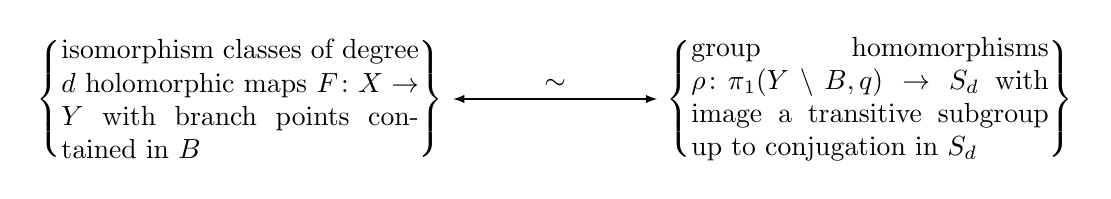
\begin{tikzpicture}[scale=1]
          \node at (-4,0) (maps)
          {
            $
              \left\{
                \begin{minipage}{30ex}
                  isomorphism classes of
                  degree $d$
                  holomorphic maps
                  $F\colon X\to Y$
                  with branch points
                  contained in $B$
                \end{minipage}
              \right\}
            $
          };
          \node at (4,0) (perms)
          {
            $
              \left\{
                \begin{minipage}{30ex}
                  group homomorphisms
                  $\rho\colon\pi_1(Y\sm B, q)\to S_d$
                  with image a transitive subgroup
                  up to conjugation in $S_d$
                \end{minipage}
              \right\}
            $
          };
          % \draw[<->] (maps) to node [above,rotate=-35] {$\sim$} node {} (perms);
          \draw[<->] (maps) to node [above] {$\sim$} node {} (perms);
        \end{tikzpicture}
      \end{center}
    \end{prop}
    If we let $Y = \PP^1$ in Proposition \ref{prop:branchedcoverofriemannsurfaces}
    and $B = \{b_1,\ldots,b_n\}\subseteq\PP^1$ we obtain
    the following correspondence:
    \begin{center}
      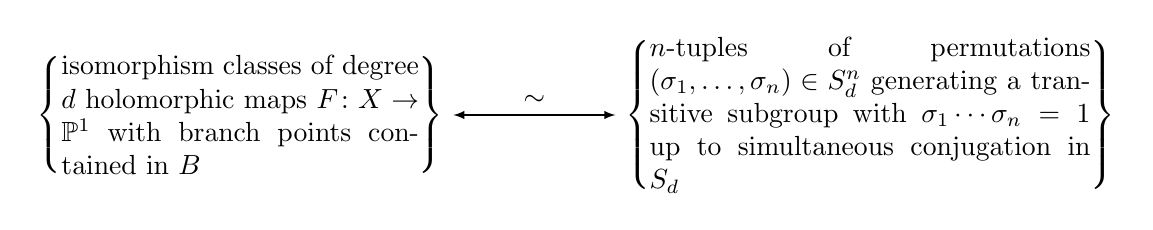
\begin{tikzpicture}[scale=1]
      \label{branchedcoverscorrespondtopermutations}
        \node at (-4,0) (maps)
        {
          $
            \left\{
              \begin{minipage}{30ex}
                isomorphism classes of
                degree $d$
                holomorphic maps
                $F\colon X\to \PP^1$
                with branch points
                contained in $B$
              \end{minipage}
            \right\}
          $
        };
        \node at (4,0) (perms)
        {
          $
            \left\{
              \begin{minipage}{37ex}
                $n$-tuples of permutations
                $(\sigma_1,\ldots,\sigma_n)\in S_d^n$
                generating a transitive subgroup
                with $\sigma_1\cdots\sigma_n=1$
                up to simultaneous conjugation in $S_d$
              \end{minipage}
            \right\}
          $
        };
        % \draw[<->] (maps) to node [above,rotate=-35] {$\sim$} node {} (perms);
        \draw[<->] (maps) to node [above] {$\sim$} node {} (perms);
      \end{tikzpicture}
    \end{center}
    Moreover,
    if $\sigma_i$ has cycle structure $(m_1,\dots,m_k)$,
    then there are $k$ preimages
    $u_1,\dots,u_k$ of $b_i$
    in the cover $F\colon X\to\PP^1$
    with $\mult_{u_j}(F) = m_j$ for all $j$.
    \begin{definition}
      \label{def:belyimapriemannsurface}
      A \defi{Belyi map} is a nonconstant holomorphic map of
      compact connected Riemann surfaces
      $F\colon X\to\PP^1$ with no more than $3$ branch points.
    \end{definition}
    \begin{definition}\label{def:galoiscover}
    \end{definition}
  }
  \section{Algebraic curves}{\label{sec:algebraiccurves}
    Let $K$ be a field isomorphic to the complex numbers,
    the real numbers, a number field, or a finite field.
    Let $\Kal$ denote an algebraic closure of $K$.
    For a detailed treatment see
    \cite[Chapters 1-2]{silverman}.
    %%%%%%%%%%%%AFFINE VARIETIES
    \begin{definition}
      \label{def:affinespace}
      \defi{Affine $n$-space} over $K$ is the
      set of $n$-tuples of elements in $\Kal$
      and denoted $\AA^n(\Kal)$ or $\AA^n$.
      % set of K-rational points of AA^n
    \end{definition}
    We will denote \defi{points} in $\AA^n$ by $P$.
    % Galois action on AA^n
    Let $\Kal[x_1,\dots,x_n]$ be the $n$-variable
    polynomial ring over $\Kal$.
    To each ideal $I\trianglelefteq\Kal[x_1,\dots,x_n]$
    we associate the following subset of $\AA^n$.
    \begin{equation}
      \label{eqn:algebraicset}
      V(I)\colonequals
      \{P\in\AA^n : f(P) = 0 \text{ for all } f\in I\}
    \end{equation}
    \begin{definition}
      \label{def:algebraicset}
      Subsets of $\AA^n$
      of the form $V(I)$ for some ideal $I$
      as in Equation \ref{eqn:algebraicset}
      are called
      \defi{affine algebraic sets}.
    \end{definition}
    Let $V$ be an affine algebraic set.
    To such a set we can associate
    the following ideal of $\Kal[x_1,\dots,x_n]$.
    \begin{equation}
      \label{eqn:idealofalgebraicset}
      I(V)\colonequals
      \{f\in\Kal[x_1,\dots,x_n]: f(P)=0 \text{ for all }f\in I\}.
    \end{equation}
    \begin{definition}
      \label{def:definedoverK}
      Let $\AA^n(K)$ denote the set of
      \defi{$K$-rational points} of $\AA^n$ defined by
      \[
        \AA^n(K)\colonequals
        \{(x_1,\dots,x_n)\in\AA^n : x_i\in K\}.
      \]
      Let $V$ be an algebraic set.
      We say $V$ is
      \defi{defined over $K$}
      if $I(V)$ can be generated by
      polynomials in $K[x_1,\dots,x_n]$.
      For such $V$ we can define the
      \defi{$K$-rational points of $V$} by
      \[
        V(K)\colonequals
        V\cap\AA^n(K).
      \]
    \end{definition}
    Let $G_K = \Gal(\Kal/K)$.
    Another way to characterize $V(K)$ is
    the points fixed under the action of $G_K$:
    \begin{equation}
      \label{eqn:galoisactiononV}
      V(K) =
      \{P\in V : P^\sigma = P\text{ for all }\sigma\in G_K\}
    \end{equation}
    \begin{definition}
      \label{def:affinevariety}
      An affine algebraic set $V$ is called
      an \defi{affine variety}
      if $I(V)\trianglelefteq\Kal[x_1,\dots,x_n]$ is a prime ideal.
    \end{definition}
    If an affine algebraic set $V$ is defined over $K$,
    then $V$ is an affine variety if
    $I(V)\trianglelefteq K[x_1,\dots,x_n]$
    is a prime ideal.
    \begin{definition}
      \label{def:coordinateringfunctionfield}
      Let $V$ be an affine variety defined over $K$.
      We define the
      \defi{affine coordinate ring}
      by
      \[
        K[V]
        \colonequals
        \frac{
          K[x_1,\dots,x_n]
        }{
        I(V)
        }
      \]
      and the
      \defi{function field of $V$}
      by the field of fractions of $K[V]$
      denoted $K(V)$.
      We can similarly define this construction
      for $\Kal[V]$ and $\Kal(V)$.
    \end{definition}
    \begin{definition}
      \label{def:dimension}
      The \defi{dimension}
      of an affine variety $V$
      is the transcendence degree of the field extension
      $\Kal(V)$ over $\Kal$.
    \end{definition}
    % \begin{definition}
    %   \label{def:nonsingular}
    %   Let $V$ be an affine variety of dimension $d$,
    %   let $P\in V$,
    %   and $I(V)$ generated by
    %   $\{f_1,\dots,f_m\}$.
    %   We say $V$ is \defi{nonsingular at $P$}
    %   if the $m\times n$ matrix of partial
    %   derivatives
    %   whose $(i,j)$-entry is
    %   \[
    %     \frac{\partial f_i}{\partial x_j}
    %   \]
    %   has rank $n-d$.
    % \end{definition}
    \begin{definition}
      \label{def:nonsingular}
      Let $V$ be a variety of dimension $d$
      and $P\in V$.
      Consider the maximal ideal
      \[
        M_P\colonequals
        \{f\in\Kal[x_1,\dots,x_n]:f(P)=0\}.
      \]
      The quotient $M_P/M_P^2$ is a finite dimensional
      vector space over $\Kal$.
      We say $P$ is \defi{nonsingular}
      if the dimension of $M_P/M_P^2$ as
      a vector space over $\Kal$
      is equal to $d$.
    \end{definition}
    \begin{definition}
      \label{def:localringatP}
      Let $V$ be an affine variety
      and $P\in V$.
      The \defi{ring of regular functions on $V$ at $P$}
      is defined to be the localization
      of $\Kal[V]$ at the maximal ideal $M_P$
      (denoted $\Kal[V]_P$).
      More explicitly we have
      \[
        \Kal[V]_P
        \colonequals
        \Kal[V]_{M_P}
        =
        \{f/g\in\Kal[V]:g(P)\neq 0\}
      \]
      so that
      the elements of
      $\Kal[V]_P$
      are well-defined
      as functions on $V$.
    \end{definition}
    %%%%%%%%%%%%PROJECTIVE VARIETIES
    \begin{definition}
      \label{def:projectivespace}
      \defi{Projective $n$-space}
      over $K$ is denoted by $\PP^n(\Kal)$
      or $\PP^n$
      and is defined to be
      \[
        \PP^n\colonequals
        \{(x_0,\dots,x_{n})\in\AA^{n+1}:\text{ not all $x_i=0$ }\}/\sim
      \]
      where
      $(x_0,\dots,x_n)\sim(x_0',\dots,x_n')$
      if there exists $\lambda\in(\Kal)^\times$ with
      $x_i=\lambda y_i$ for all $i\in \{0,\dots,n\}$.
      The equivalence class of $(x_0,\dots,x_n)\in\AA^{n+1}$
      with respect to $\sim$ is denoted by
      $[x_0,\dots,x_n]$ or $[x_0:\cdots:x_n]$.
      We call these $x_i$
      \defi{homogeneous coordinates}
      of the point in $\PP^n$.
      As in the affine case,
      we define the
      \defi{$K$-rational points} of $\PP^n$
      to be
      \[
        \PP^n(K)\colonequals
        \{[x_0,\dots,x_n]\in\PP^n:x_i\in K \text{ for all } i\}.
      \]
    \end{definition}
    \begin{definition}
      \label{def:minimalfieldofdefinitionPPn}
      Let $P\in\PP^n$ with homogeneous coordinates
      $[x_0,\dots,x_n]$.
      The \defi{minimal field of definition of $P$ over $K$}
      is
      \[
        K(P)\colonequals
        K(x_0/x_i,\dots,x_n/x_i)
      \]
      for any $i\in \{0,\dots,n\}$.
    \end{definition}
    $\PP^n(K)$ is the set of $P\in\PP^n$
    fixed by the action of $G_K$.
    On the other hand,
    $K(P)$ is the fixed field of the
    subgroup
    $\{\sigma\in G_K: P = P^\sigma\}$.
    \begin{definition}
      \label{def:homogeneousideal}
      An ideal $I\trianglelefteq\Kal[x_0,\dots,x_n]$
      is \defi{homogeneous}
      if it can be generated by homogeneous polynomials.
      To a homogeneous ideal $I$ we can associate a subset of
      $\PP^n$ as follows.
      \[
        V(I)\colonequals
        \{P\in\PP^n : f(P)=0\text{ for all homogeneous $f\in\Kal[x_0,\dots,x_n]$ }\}
      \]
      A \defi{projective algebraic set}
      is a subset of $\PP^n$ which is $V(I)$
      for some homogeneous ideal $I$.
    \end{definition}
    To any projective algebraic set $V$,
    we can associate a homogeneous ideal $I(V)$ defined by
    \begin{equation}
      \label{eqn:projectivealgebraicsetideal}
      I(V)
      \colonequals
      \{f\in\Kal[x_0,\dots,x_n]:f \text{ is homogeneous and }f(P) = 0\text{ for all $P\in V$ }\}
    \end{equation}
    % \begin{theorem}\label{thm:curvesandfunctionfields}
    %   \mm{correspondence curves and function fields}
    % \end{theorem}
    % \begin{definition}
    %   Let $K\subseteq\CC$ be a field.
    %   A \defi{branched cover of algebraic curves over $K$}
    %   is a finite map of curves
    %   $\phi\colon X\to\PP^1$ defined over $K$.
    % \end{definition}
    % \mm{enough to define good curves and function fields}
  }
  \section{Riemann's existence theorem}{\label{sec:riemannsexistence}
    Riemann surfaces are defined in Section \ref{sec:riemannsurfaces}.
    Algebraic curves are defined in Section \ref{sec:algebraiccurves}.
    Here in Section \ref{sec:riemannsexistence}
    we establish the connection between these objects over the complex numbers.
    \par
    Let $X$ be an algebraic curve over $\CC$.
    Let $\CC(t)$ denote the function field of $\PP^1$.
    By Theorem \ref{thm:curvesandfunctionfields},
    $X$ corresponds to a finite extension $L\colonequals\CC(X)$
    over $\CC(t)$.
    Let $\alpha$ be a primitive element of $L/\CC(t)$.
    Then there exists a polynomial
    \begin{equation}
      \label{eqn:minpoly}
      f(x,t) = a_0(t)+a_1(t)x+a_2(t)x^2+\cdots+a_n(t)x^n\in\CC(t)[x]
    \end{equation}
    where $f(\alpha,t) = 0$ and (after possibly clearing denominators)
    $a_i(t) \in\CC[t]$.
    The polynomial $f$ in Equation \ref{eqn:minpoly}
    defines a Riemann surface $X'$
    as a branched cover of $\PP^1$
    with branch points
    \[
      S \colonequals\left\{t_0\in\CC : f(x,t_0) \text{ has repeated roots }\right\}.
    \]
    Here $x$ can be viewed as a meromorphic function on $X'$
    and we can identify the field of meromorphic functions on $X'$
    with $L$.
    This explains how we obtain a Riemann surface from an algebraic curve.
    \par
    Suppose instead we start with a compact Riemann surface $X$.
    Can we reverse the above process to construct an algebraic curve?
    The crucial part of this process is proving that
    there exists a meromorphic function on $X$ that realizes $X$
    as a branched cover of $\PP^1$
    (see Theorem \ref{thm:riemannsexistence} below).
    Given the existence of such a function,
    the field of meromorphic functions on $X$ is then realized
    as a finite extension of the meromorphic functions on $\PP^1$.
    Finally,
    by Theorem \ref{thm:curvesandfunctionfields},
    this corresponds to an algebraic curve.
    The existence of such a function
    is given by
    Theorem \ref{thm:riemannsexistence}
    (Riemann's existence theorem).
    \begin{theorem}\label{thm:riemannsexistence}
      Let $X$ be a compact Riemann surface.
      Then there exists a meromorphic function on $X$
      that separates points.
      That is, for any set of distinct points
      $\{x_1,\dots,x_n\}\subset X$
      and any set of distinct points
      $\{t_1,\dots,t_n\}\subset\PP^1$
      there exists a meromorphic function $f$
      on $X$ such that $f(x_i) = t_i$ for all $i$.
    \end{theorem}
    \mm{todo: more details...other formulations}
  }
  \section{Belyi's theorem}{\label{sec:belyistheorem}
    In Sections
    \ref{sec:riemannsufraces}, \ref{sec:algebraiccurves},
    and \ref{sec:riemannsexistence}
    we established the equivalence between
    compact Riemann surfaces and algebraic curves over $\CC$.
    This was done, in part,
    using branched covers.
    It turns out that branched covers are the key
    to descending from the transcendental world to
    the number-theoretic world in the following sense.
    \begin{theorem}[Belyi's theorem \cite{belyi}]\label{thm:belyistheorem}
      An algebraic curve $X$ over $\CC$ can be defined over a number field
      if and only if there exists a branched cover
      $\phi\colon X\to\PP^1$ unramified outside
      $\{0,1,\infty\}$.
    \end{theorem}
    These remarkable covers are the main focus of this work.
  }
  \section{Belyi maps and Galois Belyi maps}{\label{sec:belyimaps}
    We now set up the framework to discuss
    the main mathematical objects of interest in this work.
    \begin{definition}\label{def:belyimap}
      A \defi{Belyi map}
      is a branched cover
      of algebraic curves over $\CC$
      (equivalently of Riemann surfaces)
      $\phi\colon X \to \PP^1$
      that is
      unramified outside
      $\{0,1,\infty\}$.
    \end{definition}
    \begin{definition}\label{def:belyiiso}
      Two Belyi maps
      $\phi\colon X\to\PP^1$ and
      $\phi'\colon X'\to\PP^1$
      are \defi{isomorphic}
      if there exists an isomorphism
      between $X$ and $X'$
      such that the diagram in Figure
      \ref{fig:belyiiso}
      commutes.
      If instead we only insist that the isomorphism
      makes the diagram in Figure
      \ref{fig:belyilax} commute,
      then we say that $\phi$ and $\phi'$
      are \defi{lax isomorphic}.
      \begin{figure}[ht]
        \begin{center}
          \begin{tikzcd}
            X\arrow{rr}{\sim}\arrow{dr}[swap]{\phi}&&X'\arrow{dl}{\phi'}\\
                                                   &\PP^1
          \end{tikzcd}
        \end{center}
        \caption{Belyi map isomorphism}
        \label{fig:belyiiso}
      \end{figure}
      \begin{figure}[ht]
        \begin{center}
          \begin{tikzcd}
            X\arrow{r}{\sim}\arrow{d}[swap]{\phi}&X'\arrow{d}{\phi'}\\
            \PP^1\arrow{r}{\sim}&\PP^1
          \end{tikzcd}
        \end{center}
        \caption{Belyi map lax isomorphism}
        \label{fig:belyilax}
      \end{figure}
    \end{definition}
    \begin{definition}\label{def:galoisbelyi}
      A Belyi map $\phi\colon X\to\PP^1$
      is \defi{Galois}
      if it is Galois as a cover
      (see Definition \ref{def:galoiscover}).
      A curve $X$ that admits a Galois Belyi map
      is called a \defi{Galois Belyi curve}.
    \end{definition}
    \begin{prop}\label{prop:galoiscover}
      Let $\phi\colon X\to\PP^1$ be a Galois Belyi map
      and let $\CC(X)$ be the function field of $X$.
      Then the field extension
      $\CC(X)/\CC(\PP^1)$ is Galois.
    \end{prop}
    \begin{proof}
    \end{proof}
    \begin{definition}\label{def:ramificationtype}
      The ramification
      of a degree $d$ Belyi map $\phi$
      can be encoded with $3$ partitions of $d$
      denoted $(\lambda_0,\lambda_1,\lambda_\infty)$.
      We call this triple of partitions
      the \defi{ramification type} of $\phi$.
      When $\phi$ is Galois,
      according to Lemma \ref{lem:regular},
      the ramification type of $\phi$ can more simply be encoded by
      a triple of integers $(a,b,c)\in\ZZ_{\geq 1}^3$.
    \end{definition}
    Let $\phi\colon X\to\PP^1$ be a Belyi map of degree $d$.
    Once we label the sheets of the cover
    and pick a basepoint $\star\not\in\{0,1,\infty\}$,
    we obtain a homomorphism
    \begin{equation}\label{eqn:monodromy}
      h\colon\pi_1(\PP^1\setminus\{0,1,\infty\},\star)\to S_d
    \end{equation}
    by lifting paths around the branch points of $\phi$.
    \begin{definition}\label{def:monodromy}
      The image of $h$ in Equation \ref{eqn:monodromy}
      is the \defi{monodromy group} of $\phi$
      denoted $\Mon(\phi)$.
      When $\phi$ is a Galois Belyi map,
      we can identify $\Mon(\phi)$
      as the Galois group
      $\Gal(\CC(X)/\CC(\PP^1))$.
      For this reason,
      we may also write $\Gal(\phi)$
      to denote $\Mon(\phi)$ when $\phi$
      is Galois.
    \end{definition}
    \mm{todo: any propositions about monodromy groups can go here}
    \begin{definition}\label{def:Gbelyi}
      A \defi{$G$-Galois Belyi map}
      is a Galois Belyi map
      $\phi\colon X\to\PP^1$
      with monodromy group $G$
      equipped with an isomorphism
      \[
        i\colon G\stackrel{\sim}{\to}\Mon(\phi)\leq\Aut(X).
      \]
      An \defi{isomorphism of $G$-Galois Belyi maps}
      $(\phi\colon X\to\PP^1, i\colon G\to\Mon(\phi))$
      and
      $(\phi'\colon X'\to\PP^1, i'\colon G\to\Mon(\phi)$
      is an isomorphism $h\colon X\stackrel{\sim}{\to} X'$ such that
      for all $g\in G$
      the diagram in
      Figure \ref{fig:Gbelyiiso} commutes.
      \begin{figure}[ht]
        \begin{center}
          \begin{tikzcd}
            X\arrow{rr}{h}\arrow{d}[swap]{i(g)}&&X'\arrow{d}{i'(g)}\\
            X\arrow{rr}{h}\arrow{dr}[swap]{\phi}&&X'\arrow{dl}{\phi'}\\
                                                   &\PP^1
          \end{tikzcd}
        \end{center}
        \caption{$G$-Galois Belyi map isomorphism}
        \label{fig:Gbelyiiso}
      \end{figure}
      \begin{prop}\label{prop:Gauts}
        \mm{\cite[Prop. 3.6 ish]{triangles}}
      \end{prop}
    \end{definition}
  }
  \section{Permutation triples and passports}{\label{sec:passports}
    % A \defi{(nice) curve} over $K$ is
    % a smooth, projective, geometrically connected (irreducible) scheme of finite
    % type over $K$ that is pure of dimension $1$.
    % After extension to $\CC$, a curve
    % may be thought of as a compact, connected Riemann surface.  A \defi{Belyi map}
    % over $K$ is a finite morphism $\phi\colon X \to \PP^1$ over $K$ that is
    % unramified outside $\{0,1,\infty\}$; we will sometimes write $(X,\phi)$ when we
    % want to pay special attention to the source curve $X$.  Two Belyi maps
    % $\phi,\phi'$ are \defi{isomorphic} if there is an isomorphism $\iota\colon X
    % \xrightarrow{\sim} X'$ of curves such that $\phi'\iota=\phi$.
    % Let $\phi\colon X\to\PP^1$ be a Belyi map over $\overline{\QQ}$ of degree
    % $d \in \ZZ_{\geq 1}$.
    % The \defi{monodromy group} of $\phi$ is the Galois group
    % $\Mon(\phi) \colonequals \Gal(\CC(X)\,|\,\CC(\PP^1)) \leq S_d$ of the
    % corresponding extension of function fields (understood as the action of the
    % automorphism group of the normal closure); the group $\Mon(\phi)$ may also be
    % obtained by lifting paths around $0,1,\infty$ to $X$.
    \begin{definition}
      \label{def:permutationtriple}
      A \defi{permutation triple} of degree $d \in \ZZ_{\geq 1}$ is a tuple $\sigma =
      (\sigma_0,\sigma_1,\sigma_\infty)\in S_d^3$ such that $\sigma_\infty \sigma_1
      \sigma_0 = 1$.
      A permutation triple is \defi{transitive} if the subgroup
      $\langle \sigma \rangle \leq S_d$ generated by $\sigma$ is transitive.
      We say
      that two permutation triples $\sigma,\sigma'$ are \defi{simultaneously
      conjugate} if there exists $\tau\in S_d$ such that
      \begin{equation}\label{eqn:simconj}
        \sigma^\tau \colonequals
        (\tau^{-1}\sigma_0\tau, \tau^{-1}\sigma_1\tau, \tau^{-1}\sigma_\infty\tau)
        = \left(\sigma'_0,\sigma'_1,\sigma'_\infty\right)
        = \sigma'.
      \end{equation}
      An \defi{automorphism} of a permutation triple $\sigma$ is an element of $S_d$ that
      simultaneously conjugates $\sigma$ to itself, i.e.,
      $\Aut(\sigma)=Z_{S_d}(\langle \sigma \rangle)$, the centralizer inside $S_d$.
    \end{definition}
    \begin{lemma}
      \label{lem:simulisom}
      The set of transitive permutation triples of degree $d$ up to simultaneous
      conjugation is in bijection with the set of Belyi maps of degree $d$ up to
      isomorphism.
    \end{lemma}
    \begin{proof}
      The correspondence is via monodromy \cite[Lemma 1.1]{KMSV}; in particular,
      the monodromy group of a Belyi map is (conjugate in $S_d$ to) the group
      generated by~$\sigma$.
    \end{proof}
    The group $G_\QQ\colonequals\Gal(\QQal/ \QQ)$ acts on Belyi maps by acting on the
    coefficients of a set of defining equations; under the bijection of Lemma
    \ref{lem:simulisom}, it thereby acts on the set of transitive permutation
    triples, but this action is rather mysterious.
    We can cut this action down to size by identifying some basic invariants, as
    follows.
    \begin{definition}
      \label{def:passport}
      A \defi{passport} consists of the data $\mathcal{P}=(g,G,\lambda)$
      where $g \geq 0$ is an integer, $G \leq S_d$ is a transitive subgroup, and
      $\lambda=(\lambda_0,\lambda_1,\lambda_\infty)$ is a tuple of partitions
      $\lambda_s$ of $d$ for $s=0,1,\infty$.
      These partitions will be also be
      thought of as a tuple of conjugacy classes $C=(C_0,C_1,C_\infty)$ by cycle
      type, so we will also write passports as $(g,G,C)$.
    \end{definition}
    \begin{definition}
      \label{def:passportofbelyimap}
      The \defi{passport} of a
      Belyi map $\phi\colon X \to \PP^1$ is $(g(X),\Mon(\phi),
      (\lambda_0,\lambda_1,\lambda_\infty))$,
      where $g(X)$ is the genus of $X$ and
      $\lambda_s$ is the partition of $d$ obtained by the ramification degrees above
      $s=0,1,\infty$, respectively.
    \end{definition}
    \begin{definition}
      \label{def:passportofpermutationtriple}
      The \defi{passport} of a transitive
      permutation triple $\sigma$ is
      $(g(\sigma),\langle \sigma \rangle, \lambda(\sigma))$,
      where (by Riemann--Hurwitz)
      \begin{equation}\label{eqn:riemannhurwitzfortriples}
        g(\sigma) \colonequals 1-d+(e(\sigma_0)+e(\sigma_1)+e(\sigma_\infty))/2
      \end{equation}
      and $e$ is the index of a permutation ($d$ minus the number of orbits), and
      $\lambda(\sigma)$ is the cycle type of $\sigma_s$ for $s=0,1,\infty$.
    \end{definition}
    \begin{definition}
      \label{def:passportsize}
      The
      \defi{size} of a passport $\mathcal{P}$ is the number of simultaneous conjugacy
      classes (as in \ref{eqn:simconj}) of (necessarily transitive) permutation
      triples $\sigma$ with passport $\mathcal{P}$.
    \end{definition}
    The action of $G_\QQ$ on Belyi maps preserves passports.
    Therefore, after computing equations for all Belyi maps with a given
    passport, we can try to identify the Galois orbits of this action.
    \begin{definition}
      \label{def:reduciblepassport}
      We say a passport is \defi{irreducible} if it has one
      $G_\QQ$-orbit and
      \defi{reducible} otherwise.
    \end{definition}
  }
  \section{Triangle groups}{\label{sec:trianglegroups}
    \begin{definition}
      \label{def:geometrytype}
      Let $(a,b,c)\in\ZZ_{\geq 1}^3$.
      If $1\in(a,b,c)$, then we say the triple is \defi{degenerate}.
      Otherwise, we call the triple
      \defi{spherical},
      \defi{Euclidean},
      or \defi{hyperbolic}
      according to whether the value of
      \begin{equation}
        \label{eqn:eulerchar}
        \chi(a,b,c) = 1-\frac{1}{a}-\frac{1}{b}-\frac{1}{c}
      \end{equation}
      is negative, zero, or positive.
      We call this the \defi{geometry type}
      of the triple.
      We associate the \defi{geometry}
      \begin{equation}
        \label{eqn:geometrytype}
        H=
        \begin{cases}
          \PP^1&\chi(a,b,c)<0\\
          \CC&\chi(a,b,c)=0\\
          \mathfrak{H}&\chi(a,b,c)<0
        \end{cases}
      \end{equation}
      where $\mathfrak{H}$ denotes the complex upper half-plane.
    \end{definition}
    \begin{definition}
      \label{def:trianglegroup}
      For each triple $(a,b,c)$ in Definition \ref{def:geometrytype}
      we define the \defi{triangle group}
      \begin{equation}
        \label{eqn:trianglegroup}
        \Delta(a,b,c)
        =
        \langle
        \delta_a, \delta_b, \delta_c |
        \delta_a^a=\delta_b^b=\delta_c^c=\delta_c\delta_b\delta_a=1
        \rangle
      \end{equation}
      The \defi{geometry type}
      of a triangle group $\Delta(a,b,c)$
      is the geometry type of the triple $(a,b,c)$.
    \end{definition}
    \begin{definition}\label{def:geometrytypeofbelyimap}
      The \defi{geometry type} of a Galois Belyi map
      with ramification type $(a,b,c)$
      is the geometry type of $(a,b,c)$.
    \end{definition}
    \begin{definition}\label{def:geometrytypeofpermutationtriple}
      Let $\sigma=(\sigma_0,\sigma_1,\sigma_\infty)$ be a transitive permutation triple.
      Let $a,b,c$ be the orders of
      $\sigma_0,\sigma_1,\sigma_\infty$ respectively.
      The \defi{geometry type} of $\sigma$
      is the geometry type of $(a,b,c)$.
    \end{definition}
    The connection between Belyi maps and triangle groups
    of various geometry types is explained by Lemma
    \ref{lem:belyimapsandtrianglegroups}.
    \begin{lemma}
      \label{lem:belyimapsandtrianglegroups}
      The set of isomorphism classes of of degree $d$
      Belyi maps with ramification type $(a,b,c)$
      is in bijection with the set of
      index $d$ subgroups
      $\Gamma\leq\Delta(a,b,c)$
      up to isomorphism.
    \end{lemma}
    \begin{proof}
      See \cite{KMSV} for a detailed discussion.
    \end{proof}
  }
  \section{Background results on Belyi maps}{\label{sec:backgroundresults}
    \begin{theorem}\label{thm:bigbijection}
      \mm{big bijection}
    \end{theorem}
    \begin{prop}\label{prop:galoisaction}
      \mm{Galois action on Belyi maps}
    \end{prop}
    \begin{prop}\label{prop:galoiscorrespondence}
      Galois correspondence of Belyi maps
    \end{prop}
    \begin{proof}
    \end{proof}
    \mm{\cite[1.6, 1.7]{SV}}
  }
  \section{Fields of moduli and fields of definition}{\label{sec:fieldsofmodulifieldsofdefinition}
    Let $\Aut(\CC)$ denote the field automorphisms of $\CC$.
    \begin{definition}
      \label{def:fieldofmoduli}
      Let $X$ be an algebraic curve over $\CC$.
      The \defi{field of moduli} of $X$ is the fixed field of the
      field automorphisms
      \[
        \{\tau\in\Aut(\CC) : X^\tau\cong X\}
      \]
      where $\tau\in\Aut(\CC)$ acts on the defining equations of $X$.
      Denote this field as $M(X)$.
    \end{definition}
    \begin{definition}
      \label{def:fieldofmodulibelyimap}
      Let $\phi\colon X\to\PP^1$ be a Belyi map.
      The \defi{field of moduli} of $\phi$ is the fixed field of the
      field automorphisms
      \[
        \{\tau\in\Aut(\CC) : \phi^\tau\cong \phi\}
      \]
      where $\tau\in\Aut(\CC)$ acts on the defining equations of $\phi$
      and isomorphism is determined by
      Definition \ref{def:belyiiso}.
      Denote this field as $M(\phi)$.
    \end{definition}
    \begin{definition}
      \label{def:fieldofmoduliGbelyimap}
      Let $\phi\colon X\to\PP^1$ be a $G$-Galois Belyi map.
      The \defi{field of moduli} of $\phi$ is the fixed field of the
      field automorphisms
      \[
        \{\tau\in\Aut(\CC) : \phi^\tau\cong \phi\}
      \]
      where $\tau\in\Aut(\CC)$ acts on the defining equations of $\phi$
      and isomorphism is determined by
      Definition \ref{def:Gbelyi}.
      Denote this field as $M(\phi)$.
    \end{definition}
    \begin{theorem}\label{thm:fieldofmoduli}
      Let $\phi:X\to\PP^1$ be a Belyi map
      with passport $\mathcal{P}$.
      Then the degree of the field of moduli of $\phi$
      is bounded by the size of $\mathcal{P}$.
    \end{theorem}
    \begin{proof}
      \cite{SV}
    \end{proof}
    \begin{definition}
      \label{def:fieldofdefinition}
      Let $\phi\colon X\to\PP^1$ be a Belyi map.
      A number field $K$ is a
      \defi{field of definition} for $\phi$
      if $\phi$ and $X$ can be defined
      with equations over $K$.
      If $K$ is a field of definition for $\phi$
      we say $\phi$ is \defi{defined over} $K$.
    \end{definition}
    \begin{theorem}
      \label{thm:galoisbelyimapoverfieldofmoduli}
      A Galois Belyi map is defined over
      its field of moduli.
    \end{theorem}
    \begin{proof}
      \cite[Lemma 4.1]{triangles}
    \end{proof}
  }
}
\chapter{Group theory}{\label{chapter:grouptheory}
  In this chapter we discuss results on the groups
  that arise as monodromy groups
  of the Belyi maps we are interested in.
  \section{$2$-groups}{\label{sec:twogroups}
    % def, center, exact sequence, group coho, cosets
    % examples, families: gen dihedral, gen quats, etc
    \mm{references \cite{DF}\ldots}
    Let $G$ be a finite group.
    Denote the \defi{centralizer} and
    \defi{normalizer} of a subet $S\subseteq G$
    by $C_G(S)$ and $N_G(S)$ respectively.
    Let $G$ act on a set $X$.
    For $x\in X$
    denote the \defi{stabilizer of $x$} by
    $\stab_x(G)$
    and the \defi{orbit of $x$} by
    $\orb_x(G)$.
    \begin{definition}
      \label{def:pgroup}
      Let $p$ be a rational prime.
      A finite group $G$ is a
      \defi{$p$-group}
      if the cardinality of $G$
      is a power of $p$.
    \end{definition}
    \begin{lemma}
      \label{lem:pgrouphasacenter}
      The center of a nontrivial $p$-group is nontrivial.
    \end{lemma}
    \begin{proof}
      Let $G$ be a $p$-group acting on itself by conjugation.
      Note that for $g\in G$ we have
      $C_G(g)=\stab_g(G)=N_G(\{g\})$,
      and
      $Z(G)=\cap_g C_G(g)$.
      Let
      $C_g\colonequals\orb_g(G)$
      denote the conjugacy class of $g\in G$.
      Then $\#C_g = [G:C_G(g)]$ for every $g$.
      Partitioning $G$ into conjugacy classes we obtain
      \begin{equation}\label{eqn:classequation}
        \#G =
        \#Z(G)+\sum_{i=1}^r[G:C_G(g_i)]
      \end{equation}
      where $\{g_1,\dots,g_r\}$ is a set of representatives of distinct
      conjugacy classes not contained in $Z(G)$.
      Since $g_i\not\in Z(G)$, $p$ divides $[G:C_G(g_i)]$ for every $i$.
      Then Equation \ref{eqn:classequation} implies $p$ divides
      $\#Z(G)$.
    \end{proof}
    \begin{lemma}
      \label{lem:conjugacyinsubgroups}
      Let $H$ be a normal subgroup of a $p$-group $G$.
      Let $C$ be a conjugacy class of $G$.
      Then either $C\subseteq H$ or $C\cap H = \emptyset$.
    \end{lemma}
    \begin{proof}
      Suppose $a\in C\cap H$.
      Let $x\in C$.
      Then there exists $g\in G$ so that
      $x = gag^{-1}$.
      But $a\in H$ and $H$ is normal,
      so $x=gag^{-1}\in H$.
      Thus $C\subseteq H$.
    \end{proof}
    \begin{lemma}
      \label{lem:normalimpliescentralintersect}
      Let $G$ be a $p$-group.
      Let $H$ be a nontrivial normal subgroup of $G$.
      Then $H$ intersects the center $Z(G)$ nontrivially.
    \end{lemma}
    \begin{proof}
      Let $\{g_1,\dots,g_r\}$ be a set of representatives of the
      $r$ distinct conjugacy classes (denoted $C_i$)
      of $G$ with $\#C_i\ge 2$.
      We will use Equation \ref{eqn:classequation}
      for the subgroup $H$, so
      by Lemma \ref{lem:conjugacyinsubgroups}
      we may assume all $g_i\in H$.
      The conjugacy classes of size $1$ are contained in the center $Z(G)$
      and as in Equation \ref{eqn:classequation} we
      can write
      \begin{equation}
        \label{eqn:classequationsubgroup}
        \#H = \#(H\cap Z(G))+
        \sum_{i=1}^r[G:C_G(g_i)].
      \end{equation}
      As in the proof of
      Lemma \ref{lem:pgrouphasacenter}
      we see that $p$ divides $\#(H\cap Z(G))$.
    \end{proof}
    \begin{corr}
      \label{cor:normalcentral}
      Let $H$ be a normal subgroup of order $p$ of a $p$-group $G$.
      Then $H$ is central.
    \end{corr}
    \begin{proof}
      By Lemma \ref{lem:normalimpliescentralintersect},
      $H\cap Z(G)$ is a nontrivial subgroup of $G$
      or order at least $p$.
      Since $\#H=p$ this tells us
      $H=H\cap Z(G)$.
      In particular,
      $H$ is contained in $Z(G)$.
    \end{proof}
    \begin{lemma}
      \label{lem:normalsubgroupsofallorders}
      Let $H$ be a normal subgroup of a $p$-group $G$.
      Let $\#G=p^\alpha$.
      Then $H$ contains a subgroup $H_\beta$ of order $p^\beta$
      for every divisor $p^\beta$ of $\#H$
      with the property that
      $H_\beta$ is normal in $G$ for every $\beta$.
    \end{lemma}
    \begin{proof}
    \end{proof}
    \begin{corr}
      \label{cor:normalsubgroupsofallorders}
    \end{corr}
    \begin{lemma}
      \label{lem:propersubgroupcontainedinnormalizer}
      A proper subgroup $H$ of a $p$-group $G$
      is contained in its normalizer $N_G(H)$.
    \end{lemma}
    \begin{proof}
    \end{proof}
    \begin{lemma}
      \label{lem:maximalsubgroup}
      Every maximal subgroup $H$ of a $p$-group $G$
      has $[G:H]=p$ and $H\trianglelefteq G$.
    \end{lemma}
    \begin{proof}
    \end{proof}
    \begin{definition}
      \label{def:uppercentralseries}
      Let $G$ be a finite group.
      We define a sequence of subgroups of $G$ iteratively as follows.
      Let $Z_0(G) = \{1\}$
      and let $Z_1(G) = Z(G)$.
      For $i\geq 2$ consider
      the map
      \[
        \pi\colon G\to G/Z_i(G),
      \]
      and define $Z_{i+1}(G)$ to be the preimage of the center of $G/Z_i(G)$ under $\pi$
      as follows.
      \[
        Z_{i+1}(G)\colonequals\pi^{-1}
        \left(Z\left(\frac{G}{Z_i(G)}\right)\right)
      \]
      Continuing this process produces a sequence of
      characteristic subgroups of $G$
      \[
        Z_0(G)\trianglelefteq Z_1(G)\trianglelefteq\cdots\trianglelefteq Z_{i}(G)\trianglelefteq\cdots
      \]
    \end{definition}
    \begin{definition}
      \label{def:lowercentralseries}
      For $x,y\in G$ a finite group,
      define the \defi{commutator of $x$ and $y$}
      by
      $[x,y]\colonequals x^{-1}y^{-1}xy$.
      For subgroups $H,K$ of $G$ define
      $[H,K]\colonequals\langle[h,k]:h\in H\text{ and }k\in K\rangle$.
      We define the \defi{lower central series} of $G$ iteratively as follows.
      Let $G^0=G$,
      let $G^1 = [G,G]$,
      and for $i\geq 1$ define
      $G^{i+1}=[G,G^i]$.
    \end{definition}
    \begin{definition}
      \label{def:nilpotentgroup}
      A finite group $G$ is \defi{nilpotent}
      if the upper central series
      \[
        Z_0(G)\trianglelefteq Z_1(G)\trianglelefteq\cdots\trianglelefteq Z_{i}(G)\trianglelefteq\cdots
      \]
      has $Z_c(G) = G$ for some nonnegative integer $c$.
      The integer $c$ is called the \defi{nilpotency class} of
      the nilpotent group $G$.
    \end{definition}
    \begin{lemma}
      \label{lem:upperlowernilpotent}
      % Thm 8 chapter 6.1 DF
      A finite group $G$ is nilpotent if and only if
      $G^c=\{1\}$ for some nonnegative integer $c$.
      Moreover,
      the smallest $c$ such that $G^c=\{1\}$
      is the nilpotency class of $G$ and
      \[
        Z_i(G)\leq G^{c-i-1}\leq Z_{i+1}(G)
      \]
      for all $i\in \{0,1,\dots,c-1\}$.
    \end{lemma}
    \begin{lemma}
      % Prop 2 chapter 6.1 DF
      A $p$-group of order $p^\alpha$ is nilpotent with nilpotency class
      at most $\alpha-1$.
    \end{lemma}
    \begin{proof}
    \end{proof}
    \begin{lemma}
      % Prop 7 chapter 6.1 DF
      A finite group is nilpotent if and only if
      every maximal subgroup is normal.
    \end{lemma}
    \begin{proof}
    \end{proof}
    \begin{definition}
      \label{def:frattinisubgroup}
      For a group $G$,
      define $\Phi(G)$
      to be the intersection of all maximal subgroups of $G$.
      $\Phi(G)$ is called the
      \defi{Frattini subgroup of $G$}.
    \end{definition}
  }
  \section{Examples of $2$-groups}{\label{sec:twogroupexamples}
    % examples, families: gen dihedral, gen quats, etc
  }
  \section{Cohomology modules}{\label{sec:modcoho}
    % trivial G-Module -> Cohomology module -> Holt's algorithm
  }
  \section{Iterative algorithm to produce generating triples}{\label{sec:triplesalgorithm}
  }
  \section{Description of computations}{\label{sec:grouptheorycomputations}
    % how long did it take?
    % some coarse data analysis
    % what (a,b,c) did we get
    % how many permutations, passports, (a,b,c) for each degree
    % graph distribution of genera
    % hyperbolic vs. nonhyperbolic
    % anything else you can say using just the group theory
    % Paulhus code. . .
  }
  % \section{Group theory}{
  %  \subsection{Central group extensions and $H^2(G,A)$}{
  %    \begin{definition}
  %      \label{def:isoextentions}
  %    \end{definition}
  %  }
  %  \subsection{Holt's algorithm and \texttt{Magma} implementation}{
  %    \label{subsec:holtsalgorithm}
  %  }
  %  \subsection{Results on $2$-groups}{
  %    \begin{lemma}\label{lem:2groupfiltration}
  %      \mm{todo}
  %    \end{lemma}
  %  }
  % }
}
%\chapter{Background}{\label{chapter:background}
  %  \section{What is a Belyi map?}{\label{sec:belyimaps}
  %    % \subsection{Complex manifolds, Riemann surfaces, and branched covers}{\label{subsec:riemannsurfaces}
  %    %   In Section \ref{subsec:riemannsurfaces} we outline
  %    %   basic results needed to define a ($2$-group) Belyi map
  %    %   as a holomorphic map of Riemann surfaces.
  %    %   For a more detailed discussion
  %    %   see \cite{miranda, farkas}.
  %    %   \begin{definition}
  %    %     \label{def:chart}
  %    %     A \defi{chart} on a topological space $X$
  %    %     is a homeomorphism
  %    %     $\phi\colon U\to V$
  %    %     where $U$ is an open subset of $X$
  %    %     and $V$ an open subset of $\CC$.
  %    %     We say the chart is \defi{centered}
  %    %     at $p\in U$
  %    %     if $\phi(p) = 0$.
  %    %     We say that $z = \phi(x)$ for $x\in U$
  %    %     is a \defi{local coordinate on $X$}.
  %    %   \end{definition}
  %    %   \begin{definition}
  %    %     \label{def:compatible}
  %    %     Let $\phi_1\colon U_1\to V_1$
  %    %     and $\phi_2\colon U_2\to V_2$
  %    %     be charts.
  %    %     $\phi_1$ and $\phi_2$ are
  %    %     \defi{compatible}
  %    %     if they are disjoint or
  %    %     the \defi{transition map}
  %    %     \[
  %    %       \phi_2\circ\phi_1^{-1}\colon
  %    %       \phi_1(U_1\cap U_2)\to
  %    %       \phi_2(U_1\cap U_2)
  %    %     \]
  %    %     is holomorphic.
  %    %   \end{definition}
  %    %   \begin{definition}
  %    %     \label{def:atlas}
  %    %     A \defi{complex atlas}
  %    %     on $X$ is a collection of compatible
  %    %     charts that cover $X$.
  %    %   \end{definition}
  %    %   \begin{definition}
  %    %     \label{def:equivatlas}
  %    %     Two atlases $\mathscr{A}_1$ and $\mathscr{A}_2$
  %    %     are \defi{equivalent}
  %    %     if every pair of charts
  %    %     $\phi_1, \phi_2$
  %    %     with
  %    %     $\phi_1\in\mathscr{A}_1$
  %    %     and
  %    %     $\phi_2\in\mathscr{A}_2$
  %    %     are compatible.
  %    %   \end{definition}
  %    %   \begin{definition}
  %    %     \label{def:complexstructure}
  %    %     A \defi{complex structure}
  %    %     on a topological space $X$
  %    %     is an equivalence class of atlases.
  %    %     % maximal atlas
  %    %   \end{definition}
  %    %   \begin{definition}
  %    %     \label{def:riemannsurface}
  %    %     A \defi{Riemann surface}
  %    %     is a second countable, connected,
  %    %     Hausdorff topological space $X$
  %    %     equipped with a complex structure.
  %    %   \end{definition}
  %    %   \begin{example}
  %    %     \label{exm:PP1}
  %    %     Let $\PP^1_\CC$ (or simply $\PP^1$)
  %    %     denote the set of $1$-dimensional subspaces of $\CC^2$
  %    %     which we can write as
  %    %     \[
  %    %       \{[z:w] : z,w\in\CC\text{ and }zw\ne 0\}
  %    %     \]
  %    %     where $[z:w]$ denotes the $\CC$-span of $(z,w)\in\CC^2$.
  %    %     Let $U_0 = \{[z:w]\in\PP^1 : z\neq 0\}$,
  %    %     $U_1 = \{[z:w]\in\PP^1 : w\neq 0\}$,
  %    %     define $\phi_0\colon U_0\to\CC$
  %    %     by $[z:w]\mapsto \frac{w}{z}$,
  %    %     and
  %    %     define $\phi_1\colon U_1\to\CC$
  %    %     by $[z:w]\mapsto \frac{z}{w}$.
  %    %     On $V\colonequals \phi_i(U_0\cap U_1) = \CC^\times$
  %    %     we have the holomorphic transition function
  %    %     $\phi_1\circ\phi_0^{-1}\colon V\to\CC$
  %    %     defined by $z\mapsto \frac{1}{z}$.
  %    %     The atlas consisting of these two charts $\phi_0,\phi_1$
  %    %     define a complex structure on $\PP^1$
  %    %     giving it the structure of a Riemann surface.
  %    %   \end{example}
  %    %   \begin{example}
  %    %     \label{exm:planecurves}
  %    %     \mm{plane curves and local complete intersections in $\PP^n$}
  %    %   \end{example}
  %    %   \begin{definition}
  %    %     \label{def:singularities}
  %    %     A function $f\colon X\to\CC$ is
  %    %     \defi{holomorphic
  %    %       (respectively has a removable singularity,
  %    %       has a pole, has an essential singularity)
  %    %     }
  %    %     at $p\in X$ if there exists a chart
  %    %     $\phi\colon U\to V$ such that
  %    %     $f\circ\phi^{-1}$ is
  %    %     holomorphic (respectively has a removable singularity, has a pole,
  %    %     has an essential singularity)
  %    %     at $\phi(p)$.
  %    %     $f$ is \defi{holomorphic on an open set $W\subseteq X$} if
  %    %     $f$ is holomorphic at all $p\in W$.
  %    %     $f$ is \defi{meromorphic} at $p\in X$
  %    %     if $f$ is holomorphic, has a removable singularity,
  %    %     or has a pole at $p$.
  %    %     $f$ is \defi{meromorphic on an open set $W\subseteq X$}
  %    %     if
  %    %     $f$ is meromorphic at all $p\in W$.
  %    %   \end{definition}
  %    %   % O_X(W) = {f holo on W}
  %    %   \begin{definition}
  %    %     \label{def:laurentseries}
  %    %     Let $W$ be an open subset of $X$ and denote the set of
  %    %     meromorphic functions on $W$ by
  %    %     \[
  %    %       \mathcal{M}_X(W)
  %    %       =
  %    %       \{f\colon W\to\CC : f\text{ is meromorphic on $W$ }\}.
  %    %     \]
  %    %     Let $p\in W$ and
  %    %     let $f\in\mathcal{M}_X(W)$.
  %    %     Then there exists a chart $\phi$ on $W$
  %    %     with local coordinate $z$
  %    %     and
  %    %     $\phi(p) = z_0$
  %    %     such that $f\circ\phi^{-1}$ is meromorphic at $z_0$.
  %    %     Thus,
  %    %     we can write a \defi{Laurent series expansion
  %    %     for $f\circ\phi^{-1}$}
  %    %     in a neighborhood of $z_0$
  %    %     in the local coordinate $z$
  %    %     as
  %    %     \[
  %    %       (f\circ\phi^{-1})(z) = \sum_{n}c_n(z-z_0)^n.
  %    %     \]
  %    %   \end{definition}
  %    %   \begin{definition}
  %    %     \label{def:ord}
  %    %     The minimum $n$ such that $c_n\neq 0$
  %    %     in Definition \ref{def:laurentseries}
  %    %     is the \defi{order of $f$ at $p$}
  %    %     and denoted
  %    %     $\ord_p(f)$.
  %    %   \end{definition}
  %    %   \begin{definition}
  %    %     \label{ref:holomorphicmapofRS}
  %    %     $F\colon X\to Y$ is
  %    %     \defi{holomorphic}
  %    %     at $p\in X$
  %    %     if there exists
  %    %     charts
  %    %     $\phi_1\colon U_1\to\CC$
  %    %     $\phi_2\colon U_2\to\CC$
  %    %     with $p\in U_1$ and $F(p)\in U_2$
  %    %     such that
  %    %     $\phi_2\circ F\circ\phi_1^{-1}$
  %    %     is holomorphic at $\phi_1(p)$.
  %    %     Similarly,
  %    %     $F$ is \defi{holomorphic on an open set $W\subseteq X$}
  %    %     if it is holomorphic at every $p\in W$.
  %    %   \end{definition}
  %    %   \begin{definition}
  %    %     \label{def:RSautoiso}
  %    %     An \defi{isomorphism} of Riemann surfaces is
  %    %     a bijective holomorphic map $F\colon X\to Y$
  %    %     where $F^{-1}$ is holomorphic.
  %    %     An isomorphism from $X$ to $X$ is
  %    %     an \defi{automorphism}.
  %    %   \end{definition}
  %    %   \begin{example}
  %    %     \label{exm:PP1isoCCoo}
  %    %     $\PP^1$ defined in Example
  %    %     \ref{exm:PP1}
  %    %     is isomorphic to $\CC\cup \{\infty\}$
  %    %     the compactification of the complex plane
  %    %     via stereographic projection.
  %    %   \end{example}
  %    %   \begin{theorem}
  %    %     \label{thm:compactonto}
  %    %     Let $X$ be a compact Riemann surface
  %    %     and $F\colon X\to Y$
  %    %     a nonconstant holomorphic map.
  %    %     Then $Y$ is compact an $F$ is onto.
  %    %   \end{theorem}
  %    %   \begin{prop}
  %    %     \label{prop:discretefibers}
  %    %     Let $F\colon X\to Y$ be a nonconstant
  %    %     holomorphic map of Riemann surfaces.
  %    %     Then for every $y\in Y$,
  %    %     the fiber $F^{-1}(y)$ is a discrete subset of $X$.
  %    %   \end{prop}
  %    %   % meromorphic functions on X correspond to holomorphic maps to PP1 not identically oo
  %    %   \begin{theorem}
  %    %     \label{thm:localnormalform}
  %    %     Let $F\colon X\to Y$ be a nonconstant holomorphic map.
  %    %     Let $p\in X$.
  %    %     Then there exists a positive integer $m$ such that
  %    %     for all charts
  %    %     $\phi_2$ centered at $F(p)$
  %    %     there exists a chart $\phi_1$ centered at $p$
  %    %     (let $z$ be the local coordinate)
  %    %     with $(\phi_2\circ F\circ\phi_1^{-1})(z) = z^m$.
  %    %   \end{theorem}
  %    %   \begin{definition}
  %    %     \label{def:multiplicity}
  %    %     Let $F\colon X\to Y$ be a holomorphic map
  %    %     of Riemann surfaces.
  %    %     The \defi{multiplicity}
  %    %     of $F$ at $p\in X$ is denoted
  %    %     $\mult_p(F)$ and is defined to be the unique
  %    %     integer $m$ from Theorem \ref{thm:localnormalform}
  %    %     such that there exist local coordinates about $p$
  %    %     and $F(p)$ so that
  %    %     $F$ can be written as $z\mapsto z^m$.
  %    %   \end{definition}
  %    %   \begin{definition}
  %    %     \label{def:ramificationRS}
  %    %     Let $F\colon X\to Y$ be a nonconstant holomorphic
  %    %     map of Riemann surfaces.
  %    %     $p\in X$ is a \defi{ramification point}
  %    %     of $F$
  %    %     if $\mult_p(F)\geq 2$.
  %    %     $y\in X$ is a \defi{branch point} of $F$
  %    %     if $F^{-1}(y)$ contains a ramification point.
  %    %   \end{definition}
  %    %   \begin{example}
  %    %     \label{exm:planecurve}
  %    %     \mm{plane curves, p.46, hyperelliptic curves, \ldots}
  %    %   \end{example}
  %    %   \begin{definition}
  %    %     \label{def:degreemapofRS}
  %    %     The \defi{degree}
  %    %     of a nonconstant holomorphic map
  %    %     $F\colon X\to Y$
  %    %     is
  %    %     \[
  %    %       \deg(F) \colonequals
  %    %       \sum_{p\in F^{-1}(y)}\mult_p(F)
  %    %     \]
  %    %     for any $y\in Y$.
  %    %   \end{definition}
  %    %   % sum_p ord_p(f) = 0
  %    %   \begin{theorem}[Riemann-Hurwitz]
  %    %     \label{thm:riemannhurwitzforriemannsurfaces}
  %    %     Let $F\colon X\to Y$
  %    %     be a nonconstant holomorphic map of
  %    %     compact Riemann surfaces.
  %    %     Let $g(X), g(Y)$ be the topological genus
  %    %     of $X, Y$ respectively.
  %    %     Then
  %    %     \begin{equation}
  %    %       \label{eqn:riemannhurwitzforriemannsurfaces}
  %    %       2g(X)-2=
  %    %       \deg(F)(2g(Y)-2)+
  %    %       \sum_{p\in X}(\mult_p(F)-1).
  %    %     \end{equation}
  %    %   \end{theorem}
  %    %   % groups acting on Riemann surfaces
  %    %   \begin{definition}
  %    %     \label{def:coveringspace}
  %    %     A \defi{covering space}
  %    %     of a real or complex manifold $V$
  %    %     is a continuous map
  %    %     $F\colon U\to V$ such that
  %    %     the following conditions hold:
  %    %     \begin{itemize}
  %    %       \item
  %    %         $F$ is surjective
  %    %       \item
  %    %         For all $v\in V$
  %    %         there exists a neighborhood
  %    %         $W$ of $v\in V$ such that
  %    %         $F^{-1}(W)$ consists of a disjoint
  %    %         union of open sets of $U$
  %    %         $\{U_\alpha\}_{\alpha\in I}$
  %    %         with $F|_{U_\alpha}\colon U_\alpha\to W$
  %    %         a homeomorphism.
  %    %     \end{itemize}
  %    %     The cardinality of $I$ is the \defi{degree}
  %    %     of the cover.
  %    %   \end{definition}
  %    %   \begin{definition}
  %    %     \label{def:coveringspaceiso}
  %    %     Two covering spaces $U_1\to V$
  %    %     and $U_2\to V$ are
  %    %     \defi{isomorphic}
  %    %     if there exists a homeomorphism
  %    %     $U_1\to U_2$
  %    %     making the diagram
  %    %     \begin{equation}
  %    %       \label{eqn:coveringspaceiso}
  %    %       \begin{tikzcd}
  %    %         U_1\arrow{dr}\arrow{rr}{}&&U_2\arrow{dl}\\
  %    %                        &V
  %    %       \end{tikzcd}
  %    %     \end{equation}
  %    %     commute.
  %    %   \end{definition}
  %    %   \begin{prop}
  %    %     \label{prop:universalcoveringspace}
  %    %     Given a real or complex manifold $V$,
  %    %     there exists a covering space
  %    %     $F_0\colon U_0\to V$
  %    %     such that $U_0$ is simply connected.
  %    %     $F_0$ is unique up to isomorphism
  %    %     and is universal in the following sense:
  %    %     If $F\colon U\to V$ is another cover of $V$,
  %    %     then there exists
  %    %     $G\colon U_0\to V$
  %    %     such that $F_0 = F\circ G$.
  %    %   \end{prop}
  %    %   Pick a basepoint $q\in V$
  %    %   and let $\pi_1(V,q)$ denote
  %    %   the \defi{fundamental group} of $V$
  %    %   with loops based at $q$.
  %    %   Then $\pi_1(V,q)$ acts on the cover
  %    %   $F_0\colon U_0\to V$
  %    %   via path lifting.
  %    %   % iso classes of connected covers F:U->V correspond to conj classes of subgroups of pi_1(V,q)
  %    %   We now restrict to the case of finite degree covers.
  %    %   Let $F\colon U\to V$ be a degree $d$ cover
  %    %   and consider the fiber of $q$,
  %    %   $F^{-1}(q) = \{x_1,\dots,x_n\}$.
  %    %   To a loop $\gamma$ on $V$ based at $q$,
  %    %   we can lift $\gamma$ to $d$ paths
  %    %   $\wt{\gamma}_1,\dots,\wt{\gamma}_d$
  %    %   in $U$ where $\wt{\gamma}_i$
  %    %   starts at $x_i$
  %    %   and ends at $x_j$ for some $j$.
  %    %   For each $i\in \{1,\ldots,d\}$ denote the terminal
  %    %   point of $\wt{\gamma}_i$ by $x_{\sigma(i)}\in F^{-1}(q)$.
  %    %   $\sigma$ defines
  %    %   a \defi{monodromy representation}
  %    %   \begin{equation}
  %    %     \label{eqn:monodromyrep}
  %    %     \rho\colon
  %    %     \pi_1(V,q)\to S_d.
  %    %   \end{equation}
  %    %   \begin{lemma}
  %    %     \label{lem:transitive}
  %    %     Let $\rho\colon\pi_1(V,q)\to S_d$
  %    %     be the monodromy representation
  %    %     of a
  %    %     finite degree cover $F\colon U\to V$
  %    %     with $U$ connected.
  %    %     Then the image of $\rho$
  %    %     is a transitive subgroup of $S_d$.
  %    %   \end{lemma}
  %    %   \begin{definition}
  %    %     \label{def:monodromyrepofholomorphicmap}
  %    %     Let $F\colon X\to Y$ be a nonconstant holomorphic
  %    %     map of Riemann surfaces.
  %    %     Let
  %    %     \begin{align*}
  %    %       V &\colonequals Y\sm \{\text{branch points of $F$}\}\\
  %    %       U &\colonequals X\sm \{\text{preimages of branch points of $F$}\}.
  %    %     \end{align*}
  %    %     Then $F|_U\colon U\to V$ is a covering space
  %    %     and induces a monodromy representation
  %    %     which we refer to as the
  %    %     \defi{monodromy representation of $F$}.
  %    %   \end{definition}
  %    %   \begin{definition}
  %    %     \label{def:branchedcoverofriemannsurface}
  %    %     A \defi{branched cover of Riemann surfaces} is a nonconstant holomorphic map
  %    %     of Riemann surfaces
  %    %     $\phi\colon X\to Y$ where $X$ is a compact connected Riemann surface.
  %    %   \end{definition}
  %    %   Let $Y$ be a compact connected Riemann surface,
  %    %   let $B\subseteq Y$ be a finite set,
  %    %   let $V\colonequals Y\sm B$,
  %    %   and let $F\colon U\to V$ be a finite degree cover.
  %    %   Then there is a unique complex structure on $U$
  %    %   making $F$ holomorphic.
  %    %   Let $b\in B$
  %    %   and consider a neighborhood $W$ of $b$
  %    %   small enough so that $W\sm \{b\}$ is homeomorphic to a punctured disk.
  %    %   Then $F^{-1}(W\sm \{b\})$ is a finite disjoint union
  %    %   of punctured disks $\{\wt{U}_j\}_j$.
  %    %   Moreover,
  %    %   by Theorem \ref{thm:localnormalform}
  %    %   there are integers $m_j$ for each $j$ such that
  %    %   \[
  %    %     F|_{\wt{U}_j}\colon\wt{U}_j\to W\sm \{b\}
  %    %   \]
  %    %   can be written as $z\mapsto z^{m_j}$ in local coordinates.
  %    %   Extending this holomorphic map to the unpunctured disks
  %    %   for every $b\in B$ yields the following correspondence.
  %    %   \begin{prop}
  %    %     \label{prop:branchedcoverofriemannsurfaces}
  %    %     Let $Y$ be a compact Riemann surface,
  %    %     $B\subseteq Y$ a finite set,
  %    %     and $q\in Y\sm B$ a basepoint.
  %    %     Then there is a bijection of sets
  %    %     \begin{center}
  %    %       \begin{tikzpicture}[scale=1]
  %    %         \node at (-4,0) (maps)
  %    %         {
  %    %           $
  %    %             \left\{
  %    %               \begin{minipage}{30ex}
  %    %                 isomorphism classes of
  %    %                 degree $d$
  %    %                 holomorphic maps
  %    %                 $F\colon X\to Y$
  %    %                 with branch points
  %    %                 contained in $B$
  %    %               \end{minipage}
  %    %             \right\}
  %    %           $
  %    %         };
  %    %         \node at (4,0) (perms)
  %    %         {
  %    %           $
  %    %             \left\{
  %    %               \begin{minipage}{30ex}
  %    %                 group homomorphisms
  %    %                 $\rho\colon\pi_1(Y\sm B, q)\to S_d$
  %    %                 with image a transitive subgroup
  %    %                 up to conjugation in $S_d$
  %    %               \end{minipage}
  %    %             \right\}
  %    %           $
  %    %         };
  %    %         % \draw[<->] (maps) to node [above,rotate=-35] {$\sim$} node {} (perms);
  %    %         \draw[<->] (maps) to node [above] {$\sim$} node {} (perms);
  %    %       \end{tikzpicture}
  %    %     \end{center}
  %    %   \end{prop}
  %    %   If we let $Y = \PP^1$ in Proposition \ref{prop:branchedcoverofriemannsurfaces}
  %    %   and $B = \{b_1,\ldots,b_n\}\subseteq\PP^1$ we obtain
  %    %   the following correspondence:
  %    %   \begin{center}
  %    %     \begin{tikzpicture}[scale=1]
  %    %     \label{branchedcoverscorrespondtopermutations}
  %    %       \node at (-4,0) (maps)
  %    %       {
  %    %         $
  %    %           \left\{
  %    %             \begin{minipage}{30ex}
  %    %               isomorphism classes of
  %    %               degree $d$
  %    %               holomorphic maps
  %    %               $F\colon X\to \PP^1$
  %    %               with branch points
  %    %               contained in $B$
  %    %             \end{minipage}
  %    %           \right\}
  %    %         $
  %    %       };
  %    %       \node at (4,0) (perms)
  %    %       {
  %    %         $
  %    %           \left\{
  %    %             \begin{minipage}{37ex}
  %    %               $n$-tuples of permutations
  %    %               $(\sigma_1,\ldots,\sigma_n)\in S_d^n$
  %    %               generating a transitive subgroup
  %    %               with $\sigma_1\cdots\sigma_n=1$
  %    %               up to simultaneous conjugation in $S_d$
  %    %             \end{minipage}
  %    %           \right\}
  %    %         $
  %    %       };
  %    %       % \draw[<->] (maps) to node [above,rotate=-35] {$\sim$} node {} (perms);
  %    %       \draw[<->] (maps) to node [above] {$\sim$} node {} (perms);
  %    %     \end{tikzpicture}
  %    %   \end{center}
  %    %   Moreover,
  %    %   if $\sigma_i$ has cycle structure $(m_1,\dots,m_k)$,
  %    %   then there are $k$ preimages
  %    %   $u_1,\dots,u_k$ of $b_i$
  %    %   in the cover $F\colon X\to\PP^1$
  %    %   with $\mult_{u_j}(F) = m_j$ for all $j$.
  %    %   \begin{definition}
  %    %     \label{def:belyimapriemannsurface}
  %    %     A \defi{Belyi map} is a nonconstant holomorphic map of
  %    %     compact connected Riemann surfaces
  %    %     $F\colon X\to\PP^1$ with no more than $3$ branch points.
  %    %   \end{definition}
  %    %   \begin{definition}\label{def:galoiscover}
  %    %   \end{definition}
  %    % }
  %    % \subsection{Branched covering spaces}{\label{subsec:branchedcovers}
  %    %   \mm{monodromy, ramification, Galois cover, etc}
  %    %   \begin{definition}\label{def:galoiscover}
  %    %   \end{definition}
  %    % }
  %    \subsection{Algebraic curves}{\label{subsec:algebraiccurves}
  %      Let $K$ be a field isomorphic to the complex numbers,
  %      the real numbers, a number field, or a finite field.
  %      Let $\Kal$ denote an algebraic closure of $K$.
  %      For a detailed treatment see
  %      \cite[Chapters 1-2]{silverman}.
  %      %%%%%%%%%%%%AFFINE VARIETIES
  %      \begin{definition}
  %        \label{def:affinespace}
  %        \defi{Affine $n$-space} over $K$ is the
  %        set of $n$-tuples of elements in $\Kal$
  %        and denoted $\AA^n(\Kal)$ or $\AA^n$.
  %        % set of K-rational points of AA^n
  %      \end{definition}
  %      We will denote \defi{points} in $\AA^n$ by $P$.
  %      % Galois action on AA^n
  %      Let $\Kal[x_1,\dots,x_n]$ be the $n$-variable
  %      polynomial ring over $\Kal$.
  %      To each ideal $I\trianglelefteq\Kal[x_1,\dots,x_n]$
  %      we associate the following subset of $\AA^n$.
  %      \begin{equation}
  %        \label{eqn:algebraicset}
  %        V(I)\colonequals
  %        \{P\in\AA^n : f(P) = 0 \text{ for all } f\in I\}
  %      \end{equation}
  %      \begin{definition}
  %        \label{def:algebraicset}
  %        Subsets of $\AA^n$
  %        of the form $V(I)$ for some ideal $I$
  %        as in Equation \ref{eqn:algebraicset}
  %        are called
  %        \defi{affine algebraic sets}.
  %      \end{definition}
  %      Let $V$ be an affine algebraic set.
  %      To such a set we can associate
  %      the following ideal of $\Kal[x_1,\dots,x_n]$.
  %      \begin{equation}
  %        \label{eqn:idealofalgebraicset}
  %        I(V)\colonequals
  %        \{f\in\Kal[x_1,\dots,x_n]: f(P)=0 \text{ for all }f\in I\}.
  %      \end{equation}
  %      \begin{definition}
  %        \label{def:definedoverK}
  %        Let $\AA^n(K)$ denote the set of
  %        \defi{$K$-rational points} of $\AA^n$ defined by
  %        \[
  %          \AA^n(K)\colonequals
  %          \{(x_1,\dots,x_n)\in\AA^n : x_i\in K\}.
  %        \]
  %        Let $V$ be an algebraic set.
  %        We say $V$ is
  %        \defi{defined over $K$}
  %        if $I(V)$ can be generated by
  %        polynomials in $K[x_1,\dots,x_n]$.
  %        For such $V$ we can define the
  %        \defi{$K$-rational points of $V$} by
  %        \[
  %          V(K)\colonequals
  %          V\cap\AA^n(K).
  %        \]
  %      \end{definition}
  %      Let $G_K = \Gal(\Kal/K)$.
  %      Another way to characterize $V(K)$ is
  %      the points fixed under the action of $G_K$:
  %      \begin{equation}
  %        \label{eqn:galoisactiononV}
  %        V(K) =
  %        \{P\in V : P^\sigma = P\text{ for all }\sigma\in G_K\}
  %      \end{equation}
  %      \begin{definition}
  %        \label{def:affinevariety}
  %        An affine algebraic set $V$ is called
  %        an \defi{affine variety}
  %        if $I(V)\trianglelefteq\Kal[x_1,\dots,x_n]$ is a prime ideal.
  %      \end{definition}
  %      If an affine algebraic set $V$ is defined over $K$,
  %      then $V$ is an affine variety if
  %      $I(V)\trianglelefteq K[x_1,\dots,x_n]$
  %      is a prime ideal.
  %      \begin{definition}
  %        \label{def:coordinateringfunctionfield}
  %        Let $V$ be an affine variety defined over $K$.
  %        We define the
  %        \defi{affine coordinate ring}
  %        by
  %        \[
  %          K[V]
  %          \colonequals
  %          \frac{
  %            K[x_1,\dots,x_n]
  %          }{
  %          I(V)
  %          }
  %        \]
  %        and the
  %        \defi{function field of $V$}
  %        by the field of fractions of $K[V]$
  %        denoted $K(V)$.
  %        We can similarly define this construction
  %        for $\Kal[V]$ and $\Kal(V)$.
  %      \end{definition}
  %      \begin{definition}
  %        \label{def:dimension}
  %        The \defi{dimension}
  %        of an affine variety $V$
  %        is the transcendence degree of the field extension
  %        $\Kal(V)$ over $\Kal$.
  %      \end{definition}
  %      % \begin{definition}
  %      %   \label{def:nonsingular}
  %      %   Let $V$ be an affine variety of dimension $d$,
  %      %   let $P\in V$,
  %      %   and $I(V)$ generated by
  %      %   $\{f_1,\dots,f_m\}$.
  %      %   We say $V$ is \defi{nonsingular at $P$}
  %      %   if the $m\times n$ matrix of partial
  %      %   derivatives
  %      %   whose $(i,j)$-entry is
  %      %   \[
  %      %     \frac{\partial f_i}{\partial x_j}
  %      %   \]
  %      %   has rank $n-d$.
  %      % \end{definition}
  %      \begin{definition}
  %        \label{def:nonsingular}
  %        Let $V$ be a variety of dimension $d$
  %        and $P\in V$.
  %        Consider the maximal ideal
  %        \[
  %          M_P\colonequals
  %          \{f\in\Kal[x_1,\dots,x_n]:f(P)=0\}.
  %        \]
  %        The quotient $M_P/M_P^2$ is a finite dimensional
  %        vector space over $\Kal$.
  %        We say $P$ is \defi{nonsingular}
  %        if the dimension of $M_P/M_P^2$ as
  %        a vector space over $\Kal$
  %        is equal to $d$.
  %      \end{definition}
  %      \begin{definition}
  %        \label{def:localringatP}
  %        Let $V$ be an affine variety
  %        and $P\in V$.
  %        The \defi{ring of regular functions on $V$ at $P$}
  %        is defined to be the localization
  %        of $\Kal[V]$ at the maximal ideal $M_P$
  %        (denoted $\Kal[V]_P$).
  %        More explicitly we have
  %        \[
  %          \Kal[V]_P
  %          \colonequals
  %          \Kal[V]_{M_P}
  %          =
  %          \{f/g\in\Kal[V]:g(P)\neq 0\}
  %        \]
  %        so that
  %        the elements of
  %        $\Kal[V]_P$
  %        are well-defined
  %        as functions on $V$.
  %      \end{definition}
  %      %%%%%%%%%%%%PROJECTIVE VARIETIES
  %      \begin{definition}
  %        \label{def:projectivespace}
  %        \defi{Projective $n$-space}
  %        over $K$ is denoted by $\PP^n(\Kal)$
  %        or $\PP^n$
  %        and is defined to be
  %        \[
  %          \PP^n\colonequals
  %          \{(x_0,\dots,x_{n})\in\AA^{n+1}:\text{ not all $x_i=0$ }\}/\sim
  %        \]
  %        where
  %        $(x_0,\dots,x_n)\sim(x_0',\dots,x_n')$
  %        if there exists $\lambda\in(\Kal)^\times$ with
  %        $x_i=\lambda y_i$ for all $i\in \{0,\dots,n\}$.
  %        The equivalence class of $(x_0,\dots,x_n)\in\AA^{n+1}$
  %        with respect to $\sim$ is denoted by
  %        $[x_0,\dots,x_n]$ or $[x_0:\cdots:x_n]$.
  %        We call these $x_i$
  %        \defi{homogeneous coordinates}
  %        of the point in $\PP^n$.
  %        As in the affine case,
  %        we define the
  %        \defi{$K$-rational points} of $\PP^n$
  %        to be
  %        \[
  %          \PP^n(K)\colonequals
  %          \{[x_0,\dots,x_n]\in\PP^n:x_i\in K \text{ for all } i\}.
  %        \]
  %      \end{definition}
  %      \begin{definition}
  %        \label{def:minimalfieldofdefinitionPPn}
  %        Let $P\in\PP^n$ with homogeneous coordinates
  %        $[x_0,\dots,x_n]$.
  %        The \defi{minimal field of definition of $P$ over $K$}
  %        is
  %        \[
  %          K(P)\colonequals
  %          K(x_0/x_i,\dots,x_n/x_i)
  %        \]
  %        for any $i\in \{0,\dots,n\}$.
  %      \end{definition}
  %      $\PP^n(K)$ is the set of $P\in\PP^n$
  %      fixed by the action of $G_K$.
  %      On the other hand,
  %      $K(P)$ is the fixed field of the
  %      subgroup
  %      $\{\sigma\in G_K: P = P^\sigma\}$.
  %      \begin{definition}
  %        \label{def:homogeneousideal}
  %        An ideal $I\trianglelefteq\Kal[x_0,\dots,x_n]$
  %        is \defi{homogeneous}
  %        if it can be generated by homogeneous polynomials.
  %        To a homogeneous ideal $I$ we can associate a subset of
  %        $\PP^n$ as follows.
  %        \[
  %          V(I)\colonequals
  %          \{P\in\PP^n : f(P)=0\text{ for all homogeneous $f\in\Kal[x_0,\dots,x_n]$ }\}
  %        \]
  %        A \defi{projective algebraic set}
  %        is a subset of $\PP^n$ which is $V(I)$
  %        for some homogeneous ideal $I$.
  %      \end{definition}
  %      To any projective algebraic set $V$,
  %      we can associate a homogeneous ideal $I(V)$ defined by
  %      \begin{equation}
  %        \label{eqn:projectivealgebraicsetideal}
  %        I(V)
  %        \colonequals
  %        \{f\in\Kal[x_0,\dots,x_n]:f \text{ is homogeneous and }f(P) = 0\text{ for all $P\in V$ }\}
  %      \end{equation}
  %      % \begin{theorem}\label{thm:curvesandfunctionfields}
  %      %   \mm{correspondence curves and function fields}
  %      % \end{theorem}
  %      % \begin{definition}
  %      %   Let $K\subseteq\CC$ be a field.
  %      %   A \defi{branched cover of algebraic curves over $K$}
  %      %   is a finite map of curves
  %      %   $\phi\colon X\to\PP^1$ defined over $K$.
  %      % \end{definition}
  %      % \mm{enough to define good curves and function fields}
  %    }
  %    \subsection{Riemann's existence theorem}{\label{subsec:riemannsexistence}
  %      Riemann surfaces are defined in Section \ref{subsec:riemannsurfaces}.
  %      Algebraic curves are defined in Section \ref{subsec:algebraiccurves}.
  %      Here in Section \ref{subsec:riemannsexistence}
  %      we establish the connection between these objects over the complex numbers.
  %      \par
  %      Let $X$ be an algebraic curve over $\CC$.
  %      Let $\CC(t)$ denote the function field of $\PP^1$.
  %      By Theorem \ref{thm:curvesandfunctionfields},
  %      $X$ corresponds to a finite extension $L\colonequals\CC(X)$
  %      over $\CC(t)$.
  %      Let $\alpha$ be a primitive element of $L/\CC(t)$.
  %      Then there exists a polynomial
  %      \begin{equation}
  %        \label{eqn:minpoly}
  %        f(x,t) = a_0(t)+a_1(t)x+a_2(t)x^2+\cdots+a_n(t)x^n\in\CC(t)[x]
  %      \end{equation}
  %      where $f(\alpha,t) = 0$ and (after possibly clearing denominators)
  %      $a_i(t) \in\CC[t]$.
  %      The polynomial $f$ in Equation \ref{eqn:minpoly}
  %      defines a Riemann surface $X'$
  %      as a branched cover of $\PP^1$
  %      with branch points
  %      \[
  %        S \colonequals\left\{t_0\in\CC : f(x,t_0) \text{ has repeated roots }\right\}.
  %      \]
  %      Here $x$ can be viewed as a meromorphic function on $X'$
  %      and we can identify the field of meromorphic functions on $X'$
  %      with $L$.
  %      This explains how we obtain a Riemann surface from an algebraic curve.
  %      \par
  %      Suppose instead we start with a compact Riemann surface $X$.
  %      Can we reverse the above process to construct an algebraic curve?
  %      The crucial part of this process is proving that
  %      there exists a meromorphic function on $X$ that realizes $X$
  %      as a branched cover of $\PP^1$
  %      (see Theorem \ref{thm:riemannsexistence} below).
  %      Given the existence of such a function,
  %      the field of meromorphic functions on $X$ is then realized
  %      as a finite extension of the meromorphic functions on $\PP^1$.
  %      Finally,
  %      by Theorem \ref{thm:curvesandfunctionfields},
  %      this corresponds to an algebraic curve.
  %      The existence of such a function
  %      is given by
  %      Theorem \ref{thm:riemannsexistence}
  %      (Riemann's existence theorem).
  %      \begin{theorem}\label{thm:riemannsexistence}
  %        Let $X$ be a compact Riemann surface.
  %        Then there exists a meromorphic function on $X$
  %        that separates points.
  %        That is, for any set of distinct points
  %        $\{x_1,\dots,x_n\}\subset X$
  %        and any set of distinct points
  %        $\{t_1,\dots,t_n\}\subset\PP^1$
  %        there exists a meromorphic function $f$
  %        on $X$ such that $f(x_i) = t_i$ for all $i$.
  %      \end{theorem}
  %      \mm{todo: more details...other formulations}
  %    }
  %    \subsection{Belyi's theorem}{\label{subsec:belyistheorem}
  %      In Sections
  %      \ref{subsec:riemannsufraces}, \ref{subsec:algebraiccurves},
  %      and \ref{subsec:riemannsexistence}
  %      we established the equivalence between
  %      compact Riemann surfaces and algebraic curves over $\CC$.
  %      This was done, in part,
  %      using branched covers.
  %      It turns out that branched covers are the key
  %      to descending from the transcendental world to
  %      the number-theoretic world in the following sense.
  %      \begin{theorem}[Belyi's theorem \cite{belyi}]\label{thm:belyistheorem}
  %        An algebraic curve $X$ over $\CC$ can be defined over a number field
  %        if and only if there exists a branched cover
  %        $\phi\colon X\to\PP^1$ unramified outside
  %        $\{0,1,\infty\}$.
  %      \end{theorem}
  %      These remarkable covers are the main focus of this work.
  %    }
  %    \subsection{Belyi maps and Galois Belyi maps}{\label{subsec:belyimaps}
  %      We now set up the framework to discuss
  %      the main mathematical objects of interest in this work.
  %      \begin{definition}\label{def:belyimap}
  %        A \defi{Belyi map}
  %        is a branched cover
  %        of algebraic curves over $\CC$
  %        (equivalently of Riemann surfaces)
  %        $\phi\colon X \to \PP^1$
  %        that is
  %        unramified outside
  %        $\{0,1,\infty\}$.
  %      \end{definition}
  %      \begin{definition}\label{def:belyiiso}
  %        Two Belyi maps
  %        $\phi\colon X\to\PP^1$ and
  %        $\phi'\colon X'\to\PP^1$
  %        are \defi{isomorphic}
  %        if there exists an isomorphism
  %        between $X$ and $X'$
  %        such that the diagram in Figure
  %        \ref{fig:belyiiso}
  %        commutes.
  %        If instead we only insist that the isomorphism
  %        makes the diagram in Figure
  %        \ref{fig:belyilax} commute,
  %        then we say that $\phi$ and $\phi'$
  %        are \defi{lax isomorphic}.
  %        \begin{figure}[ht]
  %          \begin{center}
  %            \begin{tikzcd}
  %              X\arrow{rr}{\sim}\arrow{dr}[swap]{\phi}&&X'\arrow{dl}{\phi'}\\
  %                                                     &\PP^1
  %            \end{tikzcd}
  %          \end{center}
  %          \caption{Belyi map isomorphism}
  %          \label{fig:belyiiso}
  %        \end{figure}
  %        \begin{figure}[ht]
  %          \begin{center}
  %            \begin{tikzcd}
  %              X\arrow{r}{\sim}\arrow{d}[swap]{\phi}&X'\arrow{d}{\phi'}\\
  %              \PP^1\arrow{r}{\sim}&\PP^1
  %            \end{tikzcd}
  %          \end{center}
  %          \caption{Belyi map lax isomorphism}
  %          \label{fig:belyilax}
  %        \end{figure}
  %      \end{definition}
  %      \begin{definition}\label{def:galoisbelyi}
  %        A Belyi map $\phi\colon X\to\PP^1$
  %        is \defi{Galois}
  %        if it is Galois as a cover
  %        (see Definition \ref{def:galoiscover}).
  %        A curve $X$ that admits a Galois Belyi map
  %        is called a \defi{Galois Belyi curve}.
  %      \end{definition}
  %      \begin{prop}\label{prop:galoiscover}
  %        Let $\phi\colon X\to\PP^1$ be a Galois Belyi map
  %        and let $\CC(X)$ be the function field of $X$.
  %        Then the field extension
  %        $\CC(X)/\CC(\PP^1)$ is Galois.
  %      \end{prop}
  %      \begin{proof}
  %      \end{proof}
  %      \begin{definition}\label{def:ramificationtype}
  %        The ramification
  %        of a degree $d$ Belyi map $\phi$
  %        can be encoded with $3$ partitions of $d$
  %        denoted $(\lambda_0,\lambda_1,\lambda_\infty)$.
  %        We call this triple of partitions
  %        the \defi{ramification type} of $\phi$.
  %        When $\phi$ is Galois,
  %        according to Lemma \ref{lem:regular},
  %        the ramification type of $\phi$ can more simply be encoded by
  %        a triple of integers $(a,b,c)\in\ZZ_{\geq 1}^3$.
  %      \end{definition}
  %      Let $\phi\colon X\to\PP^1$ be a Belyi map of degree $d$.
  %      Once we label the sheets of the cover
  %      and pick a basepoint $\star\not\in\{0,1,\infty\}$,
  %      we obtain a homomorphism
  %      \begin{equation}\label{eqn:monodromy}
  %        h\colon\pi_1(\PP^1\setminus\{0,1,\infty\},\star)\to S_d
  %      \end{equation}
  %      by lifting paths around the branch points of $\phi$.
  %      \begin{definition}\label{def:monodromy}
  %        The image of $h$ in Equation \ref{eqn:monodromy}
  %        is the \defi{monodromy group} of $\phi$
  %        denoted $\Mon(\phi)$.
  %        When $\phi$ is a Galois Belyi map,
  %        we can identify $\Mon(\phi)$
  %        as the Galois group
  %        $\Gal(\CC(X)/\CC(\PP^1))$.
  %        For this reason,
  %        we may also write $\Gal(\phi)$
  %        to denote $\Mon(\phi)$ when $\phi$
  %        is Galois.
  %      \end{definition}
  %      \mm{todo: any propositions about monodromy groups can go here}
  %      \begin{definition}\label{def:Gbelyi}
  %        A \defi{$G$-Galois Belyi map}
  %        is a Galois Belyi map
  %        $\phi\colon X\to\PP^1$
  %        with monodromy group $G$
  %        equipped with an isomorphism
  %        \[
  %          i\colon G\stackrel{\sim}{\to}\Mon(\phi)\leq\Aut(X).
  %        \]
  %        An \defi{isomorphism of $G$-Galois Belyi maps}
  %        $(\phi\colon X\to\PP^1, i\colon G\to\Mon(\phi))$
  %        and
  %        $(\phi'\colon X'\to\PP^1, i'\colon G\to\Mon(\phi)$
  %        is an isomorphism $h\colon X\stackrel{\sim}{\to} X'$ such that
  %        for all $g\in G$
  %        the diagram in
  %        Figure \ref{fig:Gbelyiiso} commutes.
  %        \begin{figure}[ht]
  %          \begin{center}
  %            \begin{tikzcd}
  %              X\arrow{rr}{h}\arrow{d}[swap]{i(g)}&&X'\arrow{d}{i'(g)}\\
  %              X\arrow{rr}{h}\arrow{dr}[swap]{\phi}&&X'\arrow{dl}{\phi'}\\
  %                                                     &\PP^1
  %            \end{tikzcd}
  %          \end{center}
  %          \caption{$G$-Galois Belyi map isomorphism}
  %          \label{fig:Gbelyiiso}
  %        \end{figure}
  %        \begin{prop}\label{prop:Gauts}
  %          \mm{\cite[Prop. 3.6 ish]{triangles}}
  %        \end{prop}
  %      \end{definition}
  %    }
  %    \subsection{Permutation triples and passports}{\label{subsec:passports}
  %      % A \defi{(nice) curve} over $K$ is
  %      % a smooth, projective, geometrically connected (irreducible) scheme of finite
  %      % type over $K$ that is pure of dimension $1$.
  %      % After extension to $\CC$, a curve
  %      % may be thought of as a compact, connected Riemann surface.  A \defi{Belyi map}
  %      % over $K$ is a finite morphism $\phi\colon X \to \PP^1$ over $K$ that is
  %      % unramified outside $\{0,1,\infty\}$; we will sometimes write $(X,\phi)$ when we
  %      % want to pay special attention to the source curve $X$.  Two Belyi maps
  %      % $\phi,\phi'$ are \defi{isomorphic} if there is an isomorphism $\iota\colon X
  %      % \xrightarrow{\sim} X'$ of curves such that $\phi'\iota=\phi$.
  %      % Let $\phi\colon X\to\PP^1$ be a Belyi map over $\overline{\QQ}$ of degree
  %      % $d \in \ZZ_{\geq 1}$.
  %      % The \defi{monodromy group} of $\phi$ is the Galois group
  %      % $\Mon(\phi) \colonequals \Gal(\CC(X)\,|\,\CC(\PP^1)) \leq S_d$ of the
  %      % corresponding extension of function fields (understood as the action of the
  %      % automorphism group of the normal closure); the group $\Mon(\phi)$ may also be
  %      % obtained by lifting paths around $0,1,\infty$ to $X$.
  %      \begin{definition}
  %        \label{def:permutationtriple}
  %        A \defi{permutation triple} of degree $d \in \ZZ_{\geq 1}$ is a tuple $\sigma =
  %        (\sigma_0,\sigma_1,\sigma_\infty)\in S_d^3$ such that $\sigma_\infty \sigma_1
  %        \sigma_0 = 1$.
  %        A permutation triple is \defi{transitive} if the subgroup
  %        $\langle \sigma \rangle \leq S_d$ generated by $\sigma$ is transitive.
  %        We say
  %        that two permutation triples $\sigma,\sigma'$ are \defi{simultaneously
  %        conjugate} if there exists $\tau\in S_d$ such that
  %        \begin{equation}\label{eqn:simconj}
  %          \sigma^\tau \colonequals
  %          (\tau^{-1}\sigma_0\tau, \tau^{-1}\sigma_1\tau, \tau^{-1}\sigma_\infty\tau)
  %          = \left(\sigma'_0,\sigma'_1,\sigma'_\infty\right)
  %          = \sigma'.
  %        \end{equation}
  %        An \defi{automorphism} of a permutation triple $\sigma$ is an element of $S_d$ that
  %        simultaneously conjugates $\sigma$ to itself, i.e.,
  %        $\Aut(\sigma)=Z_{S_d}(\langle \sigma \rangle)$, the centralizer inside $S_d$.
  %      \end{definition}
  %      \begin{lemma}
  %        \label{lem:simulisom}
  %        The set of transitive permutation triples of degree $d$ up to simultaneous
  %        conjugation is in bijection with the set of Belyi maps of degree $d$ up to
  %        isomorphism.
  %      \end{lemma}
  %      \begin{proof}
  %        The correspondence is via monodromy \cite[Lemma 1.1]{KMSV}; in particular,
  %        the monodromy group of a Belyi map is (conjugate in $S_d$ to) the group
  %        generated by~$\sigma$.
  %      \end{proof}
  %      The group $G_\QQ\colonequals\Gal(\QQal/ \QQ)$ acts on Belyi maps by acting on the
  %      coefficients of a set of defining equations; under the bijection of Lemma
  %      \ref{lem:simulisom}, it thereby acts on the set of transitive permutation
  %      triples, but this action is rather mysterious.
  %      We can cut this action down to size by identifying some basic invariants, as
  %      follows.
  %      \begin{definition}
  %        \label{def:passport}
  %        A \defi{passport} consists of the data $\mathcal{P}=(g,G,\lambda)$
  %        where $g \geq 0$ is an integer, $G \leq S_d$ is a transitive subgroup, and
  %        $\lambda=(\lambda_0,\lambda_1,\lambda_\infty)$ is a tuple of partitions
  %        $\lambda_s$ of $d$ for $s=0,1,\infty$.
  %        These partitions will be also be
  %        thought of as a tuple of conjugacy classes $C=(C_0,C_1,C_\infty)$ by cycle
  %        type, so we will also write passports as $(g,G,C)$.
  %      \end{definition}
  %      \begin{definition}
  %        \label{def:passportofbelyimap}
  %        The \defi{passport} of a
  %        Belyi map $\phi\colon X \to \PP^1$ is $(g(X),\Mon(\phi),
  %        (\lambda_0,\lambda_1,\lambda_\infty))$,
  %        where $g(X)$ is the genus of $X$ and
  %        $\lambda_s$ is the partition of $d$ obtained by the ramification degrees above
  %        $s=0,1,\infty$, respectively.
  %      \end{definition}
  %      \begin{definition}
  %        \label{def:passportofpermutationtriple}
  %        The \defi{passport} of a transitive
  %        permutation triple $\sigma$ is
  %        $(g(\sigma),\langle \sigma \rangle, \lambda(\sigma))$,
  %        where (by Riemann--Hurwitz)
  %        \begin{equation}\label{eqn:riemannhurwitzfortriples}
  %          g(\sigma) \colonequals 1-d+(e(\sigma_0)+e(\sigma_1)+e(\sigma_\infty))/2
  %        \end{equation}
  %        and $e$ is the index of a permutation ($d$ minus the number of orbits), and
  %        $\lambda(\sigma)$ is the cycle type of $\sigma_s$ for $s=0,1,\infty$.
  %      \end{definition}
  %      \begin{definition}
  %        \label{def:passportsize}
  %        The
  %        \defi{size} of a passport $\mathcal{P}$ is the number of simultaneous conjugacy
  %        classes (as in \ref{eqn:simconj}) of (necessarily transitive) permutation
  %        triples $\sigma$ with passport $\mathcal{P}$.
  %      \end{definition}
  %      The action of $G_\QQ$ on Belyi maps preserves passports.
  %      Therefore, after computing equations for all Belyi maps with a given
  %      passport, we can try to identify the Galois orbits of this action.
  %      \begin{definition}
  %        \label{def:reduciblepassport}
  %        We say a passport is \defi{irreducible} if it has one
  %        $G_\QQ$-orbit and
  %        \defi{reducible} otherwise.
  %      \end{definition}
  %    }
  %    \subsection{Triangle groups}{\label{subsec:trianglegroups}
  %      \begin{definition}
  %        \label{def:geometrytype}
  %        Let $(a,b,c)\in\ZZ_{\geq 1}^3$.
  %        If $1\in(a,b,c)$, then we say the triple is \defi{degenerate}.
  %        Otherwise, we call the triple
  %        \defi{spherical},
  %        \defi{Euclidean},
  %        or \defi{hyperbolic}
  %        according to whether the value of
  %        \begin{equation}
  %          \label{eqn:eulerchar}
  %          \chi(a,b,c) = 1-\frac{1}{a}-\frac{1}{b}-\frac{1}{c}
  %        \end{equation}
  %        is negative, zero, or positive.
  %        We call this the \defi{geometry type}
  %        of the triple.
  %        We associate the \defi{geometry}
  %        \begin{equation}
  %          \label{eqn:geometrytype}
  %          H=
  %          \begin{cases}
  %            \PP^1&\chi(a,b,c)<0\\
  %            \CC&\chi(a,b,c)=0\\
  %            \mathfrak{H}&\chi(a,b,c)<0
  %          \end{cases}
  %        \end{equation}
  %        where $\mathfrak{H}$ denotes the complex upper half-plane.
  %      \end{definition}
  %      \begin{definition}
  %        \label{def:trianglegroup}
  %        For each triple $(a,b,c)$ in Definition \ref{def:geometrytype}
  %        we define the \defi{triangle group}
  %        \begin{equation}
  %          \label{eqn:trianglegroup}
  %          \Delta(a,b,c)
  %          =
  %          \langle
  %          \delta_a, \delta_b, \delta_c |
  %          \delta_a^a=\delta_b^b=\delta_c^c=\delta_c\delta_b\delta_a=1
  %          \rangle
  %        \end{equation}
  %        The \defi{geometry type}
  %        of a triangle group $\Delta(a,b,c)$
  %        is the geometry type of the triple $(a,b,c)$.
  %      \end{definition}
  %      \begin{definition}\label{def:geometrytypeofbelyimap}
  %        The \defi{geometry type} of a Galois Belyi map
  %        with ramification type $(a,b,c)$
  %        is the geometry type of $(a,b,c)$.
  %      \end{definition}
  %      \begin{definition}\label{def:geometrytypeofpermutationtriple}
  %        Let $\sigma=(\sigma_0,\sigma_1,\sigma_\infty)$ be a transitive permutation triple.
  %        Let $a,b,c$ be the orders of
  %        $\sigma_0,\sigma_1,\sigma_\infty$ respectively.
  %        The \defi{geometry type} of $\sigma$
  %        is the geometry type of $(a,b,c)$.
  %      \end{definition}
  %      The connection between Belyi maps and triangle groups
  %      of various geometry types is explained by Lemma
  %      \ref{lem:belyimapsandtrianglegroups}.
  %      \begin{lemma}
  %        \label{lem:belyimapsandtrianglegroups}
  %        The set of isomorphism classes of of degree $d$
  %        Belyi maps with ramification type $(a,b,c)$
  %        is in bijection with the set of
  %        index $d$ subgroups
  %        $\Gamma\leq\Delta(a,b,c)$
  %        up to isomorphism.
  %      \end{lemma}
  %      \begin{proof}
  %        See \cite{KMSV} for a detailed discussion.
  %      \end{proof}
  %    }
  %    \subsection{Background results on Belyi maps}{\label{subsec:backgroundresults}
  %      \begin{theorem}\label{thm:bigbijection}
  %        \mm{big bijection}
  %      \end{theorem}
  %      \begin{prop}\label{prop:galoisaction}
  %        \mm{Galois action on Belyi maps}
  %      \end{prop}
  %      \begin{prop}\label{prop:galoiscorrespondence}
  %        Galois correspondence of Belyi maps
  %      \end{prop}
  %      \begin{proof}
  %      \end{proof}
  %      \mm{\cite[1.6, 1.7]{SV}}
  %    }
  %    \subsection{Fields of moduli and fields of definition}{\label{subsec:fieldsofmodulifieldsofdefinition}
  %      Let $\Aut(\CC)$ denote the field automorphisms of $\CC$.
  %      \begin{definition}
  %        \label{def:fieldofmoduli}
  %        Let $X$ be an algebraic curve over $\CC$.
  %        The \defi{field of moduli} of $X$ is the fixed field of the
  %        field automorphisms
  %        \[
  %          \{\tau\in\Aut(\CC) : X^\tau\cong X\}
  %        \]
  %        where $\tau\in\Aut(\CC)$ acts on the defining equations of $X$.
  %        Denote this field as $M(X)$.
  %      \end{definition}
  %      \begin{definition}
  %        \label{def:fieldofmodulibelyimap}
  %        Let $\phi\colon X\to\PP^1$ be a Belyi map.
  %        The \defi{field of moduli} of $\phi$ is the fixed field of the
  %        field automorphisms
  %        \[
  %          \{\tau\in\Aut(\CC) : \phi^\tau\cong \phi\}
  %        \]
  %        where $\tau\in\Aut(\CC)$ acts on the defining equations of $\phi$
  %        and isomorphism is determined by
  %        Definition \ref{def:belyiiso}.
  %        Denote this field as $M(\phi)$.
  %      \end{definition}
  %      \begin{definition}
  %        \label{def:fieldofmoduliGbelyimap}
  %        Let $\phi\colon X\to\PP^1$ be a $G$-Galois Belyi map.
  %        The \defi{field of moduli} of $\phi$ is the fixed field of the
  %        field automorphisms
  %        \[
  %          \{\tau\in\Aut(\CC) : \phi^\tau\cong \phi\}
  %        \]
  %        where $\tau\in\Aut(\CC)$ acts on the defining equations of $\phi$
  %        and isomorphism is determined by
  %        Definition \ref{def:Gbelyi}.
  %        Denote this field as $M(\phi)$.
  %      \end{definition}
  %      \begin{theorem}\label{thm:fieldofmoduli}
  %        Let $\phi:X\to\PP^1$ be a Belyi map
  %        with passport $\mathcal{P}$.
  %        Then the degree of the field of moduli of $\phi$
  %        is bounded by the size of $\mathcal{P}$.
  %      \end{theorem}
  %      \begin{proof}
  %        \cite{SV}
  %      \end{proof}
  %      \begin{definition}
  %        \label{def:fieldofdefinition}
  %        Let $\phi\colon X\to\PP^1$ be a Belyi map.
  %        A number field $K$ is a
  %        \defi{field of definition} for $\phi$
  %        if $\phi$ and $X$ can be defined
  %        with equations over $K$.
  %        If $K$ is a field of definition for $\phi$
  %        we say $\phi$ is \defi{defined over} $K$.
  %      \end{definition}
  %      \begin{theorem}
  %        \label{thm:galoisbelyimapoverfieldofmoduli}
  %        A Galois Belyi map is defined over
  %        its field of moduli.
  %      \end{theorem}
  %      \begin{proof}
  %        \cite[Lemma 4.1]{triangles}
  %      \end{proof}
  %    }
  %  }
  %  \section{Group theory}{
  %    \subsection{Central group extensions and $H^2(G,A)$}{
  %      \begin{definition}
  %        \label{def:isoextentions}
  %      \end{definition}
  %    }
  %    \subsection{Holt's algorithm and \texttt{Magma} implementation}{
  %      \label{subsec:holtsalgorithm}
  %    }
  %    \subsection{Results on $2$-groups}{
  %      \begin{lemma}\label{lem:2groupfiltration}
  %        \mm{todo}
  %      \end{lemma}
  %    }
  %  }
  %  % \section{Jacobians of curves}{
  %  %   \subsection{Abel-Jacobi and the construction over $\CC$}{
  %  %   }
  %  %   \subsection{Algebraic construction}{
  %  %   }
  %  %   \subsection{Riemann-Roch}{
  %  %   }
  %  %   \subsection{Torsion points and torsion fields}{
  %  %   }
  %  % }
  %  % \section{Galois representations}{
  %  %   \subsection{Representations of Galois groups of number fields}{
  %  %   }
  %  %   \subsection{Representations coming from geometry}{
  %  %   }
  %  % }
%}
\chapter{A database of $2$-group Belyi maps}{\label{chapter:database}
  In this chapter we describe an algorithm
  to generate $2$-group Belyi maps of a given degree.
  The algorithm is inductive in the degree.
  The base case in degree $1$ is discussed in Section \ref{sec:degree1}.
  We then move on to describe the inductive step of the algorithm
  which we describe in two parts.
  First we discuss the algorithm to enumerate the isomorphism classes
  using permutation triples in Section \ref{sec:isoclasses}.
  For a discussion on the relationship between permutation triples and Belyi maps
  see Section \ref{sec:belyimaps}.
  Next we discuss the inductive step to produce Belyi curves and maps in Section \ref{sec:curvesandmaps}.
  In Section \ref{sec:runtime} we give a detailed description of the running time of the algorithm.
  Lastly,
  in Section \ref{sec:computations},
  we discuss the implementation and computations that we have carried out explicitly.
  Recall the definition of a $G$-Galois Belyi map in Section \ref{sec:belyimaps}.
  In this section we narrow our focus
  to $G$-Galois Belyi maps with $\#G$ a power of $2$.
  \begin{definition}\label{def:2groupbelyi}
    A \defi{$2$-group Belyi map} is a Galois Belyi map
    with monodromy group a $2$-group.
  \end{definition}
  \section{Degree $1$ Belyi maps}{\label{sec:degree1}
  }
  \section{An algorithm to enumerate isomorphism classes of $2$-group Belyi maps}{\label{sec:isoclasses}
    The algorithm we describe here is iterative.
    The degree $1$ case is discussed in Section \ref{sec:degree1}.
    We now set up some notation for the iteration.
    \begin{notation}\label{not:triples}
      First we suppose that we are given
      $\sigma$ a permutation triple corresponding
      to a $2$-group Belyi map $\phi:X\to\PP^1$.
      \begin{definition}
        \label{def:lift}
        We say that a permutation triple $\wt{\sigma}$
        is a \defi{degree $2$ lift} (or simply a \defi{lift})
        of a permutation triple $\sigma$ if
        there exists a short exact sequence of groups
        as in Figure \ref{fig:lifttriple}
        with $\iota(\ZZ/2\ZZ)$ contained in the center of
        $\langle\wt{\sigma}\rangle$.
      \end{definition}
      \begin{figure}[ht]\label{fig:lifttriple}
        \[
          \begin{tikzcd}[ampersand replacement=\&, row sep = small]
            1\arrow{r}\&\ZZ/2\ZZ\arrow{r}{\iota}\&\langle\widetilde{\sigma}\rangle\arrow{r}{\pi}\&\langle\sigma\rangle\arrow{r}\&1
          \end{tikzcd}
        \]
        \caption{$\wt{\sigma}$ a lift of $\sigma$}
      \end{figure}
      In Algorithm \ref{alg:triples} below
      we describe how to determine all lifts $\wt{\sigma}$ (up to isomorphism)
      of a given permutation triple $\sigma$.
      \begin{lemma}
        \label{lem:central}
        Let $\sigma$ be a permutation triple corresponding to a $2$-group Belyi map
        $\phi:X\to\PP^1$ and $\wt{\sigma}$ a lift of $\sigma$
        corresponding to a $2$-group Belyi map $\wt{\phi}:\wt{X}\to\PP^1$.
        Then there exists a permutation triple $\wt{\sigma}'$
        that is simultaneously conjugate to $\wt{\sigma}$ with
        $\iota(\langle\wt{\sigma}'\rangle)$ contained in the center of
        $\langle\sigma\rangle$.
      \end{lemma}
      \begin{proof}
      \end{proof}
      \begin{remark}
        \label{rmk:central}
        In light of Lemma \ref{lem:central},
        we can restrict our attention to central extensions of
        $\langle\sigma\rangle$
        in Definition \ref{def:lift}.
      \end{remark}
    \end{notation}
    \begin{alg}\label{alg:triples}
      Let the notation be as described above in \ref{not:triples}.
      \newline
      \textbf{Input}: $\sigma=(\sigma_0,\sigma_1,\sigma_\infty)\in S_d^3$ a permutation triple
      corresponding to a $2$-group Belyi map
      \newline
      \textbf{Output}: all lifts $\wt{\sigma}$
      of $\sigma$ up to simultaneous conjugation in $S_{2d}$
      \begin{enumerate}
        \item
          Let $G = \langle\sigma\rangle$
          and compute all central extensions $\wt{G}$
          sitting in the exact sequence in Figure \ref{fig:centralext}
          up to isomorphism (see Definition \ref{def:isoextentions}).
          For more information about the algorithms to do this
          see Section \ref{subsec:holtsalgorithm}.
          \begin{figure}[ht]
            \[
              \begin{tikzcd}[ampersand replacement=\&, row sep = small]
                1\arrow{r}\&\ZZ/2\ZZ\arrow{r}{\iota}\&\wt{G}\arrow{r}{\pi}\&G\arrow{r}\&1
              \end{tikzcd}
            \]
            \caption{$\wt{G}$ a (central) extension of $G$}
            \label{fig:centralext}
          \end{figure}
        \item
          For each extension $\wt{G}$ as in Figure \ref{fig:centralext}
          from the previous step
          we perform the following:
          \begin{enumerate}
            \item
              % For $s\in\{0,1,\infty\}$,
              % $\sigma_s$ has $2$ preimages under the map $\pi$
              % which yields $8$ triples $\wt{\sigma} = (\wt{\sigma}_0,\wt{\sigma}_1,\wt{\sigma}_\infty)$
              % with the property that $\pi(\wt{\sigma}_s) = \sigma_s$ for each $s$.
              Consider the set of triples
              \begin{equation}
                \label{eqn:lifts}
                \{
                  \wt{\sigma}\colonequals(\wt{\sigma}_0, \wt{\sigma}_1, \wt{\sigma}_\infty) :
                  \wt{\sigma}_s\in\pi^{-1}(\sigma_s)\text{ for }
                  s\in\{0,1,\infty\}
                \}
              \end{equation}
              and let $\Lifts(\sigma)$ denote the set of such $\wt{\sigma}$
              with the property that $\wt{\sigma}_\infty\wt{\sigma}_1\wt{\sigma}_0 = 1$
              and $\langle\wt{\sigma}\rangle = \wt{G}$.
            \item
              For each $\wt{\sigma}\in\Lifts(\sigma)$ compute
              $\order(\wt{\sigma})\colonequals(\order(\wt{\sigma}_0), \order(\wt{\sigma}_1), \order(\wt{\sigma}_\infty))\in\ZZ^3$
              and sort $\Lifts(\sigma)$ according to $\order(\wt{\sigma})$.
              Let
              \begin{equation}
                \label{eqn:liftsorders}
                \Lifts(\sigma,(a,b,c))\colonequals
                \{
                  \wt{\sigma}\in\Lifts(\sigma) :
                  \order(\wt{\sigma}) = (a,b,c)
                \}.
              \end{equation}
            \item
              For each set of triples $\Lifts(\sigma,(a,b,c))$
              remove simultaneously conjugate triples so that
              $\Lifts(\sigma,(a,b,c))$ has exactly one representative
              from each simultaneous conjugacy class.
              \mm{TODO: reword}
          \end{enumerate}
        \item
          Return the union of the sets $\Lifts(\sigma,(a,b,c))$
          ranging over all extensions as in Figure
          \ref{fig:centralext}
          and for each extension ranging over all orders
          $(a,b,c)$.
      \end{enumerate}
    \end{alg}
    \begin{proof}[Proof of correctness]
      The algorithms in Step 1 are addressed in Section \ref{subsec:holtsalgorithm}.
      Let $\phi:X\to\PP^1$ be the $2$-group Belyi map corresponding to $\sigma$.
      By Proposition \ref{prop:galoiscorrespondence},
      the groups obtained from Step 1 are precisely the
      groups that can occur as monodromy groups of degree $2$ covers of $X$.
      \mm{
        lemma in section about extensions
        (or in background about Belyi maps)
        to prove
        that two isomorphic extensions cannot produce
        nonisomorphic Belyi maps
        and that two nonisomorphic extensions cannot produce
        isomorphic Belyi maps
      }
      In Step 2 we restrict our attention to a single extension of $G$
      as in Figure \ref{fig:centralext}.
      When we pullback a triple $\sigma$ under the map $\pi$,
      there are $2^3=8$ preimages $\wt{\sigma}$.
      Of these $8$ preimages, exactly $4$ have the property that
      $\wt{\sigma}_\infty\wt{\sigma}_1\wt{\sigma}_0=1$.
      Of these $4$ triples, we only take those that generate $\wt{G}$
      and this makes up the set $\Lifts(\sigma)$.
      In Step 2(b),
      we are sorting $\Lifts(\sigma)$ by passport.
      Since $2$-group Belyi maps are Galois,
      the cycle structure of each $\wt{\sigma}_s\in\wt{\sigma}$
      is determined by the order of $\wt{\sigma}_s$
      so that sorting by order is the same as sorting by cycle structure.
      \begin{remark}\label{rmk:twouniquepassports}
        In fact,
        even though we do not need this for the algorithm,
        there are at most $2$ different passports that can occur
        in $\Lifts(\sigma)$.
        $2$ different passports occur when one of $\sigma_s\in\sigma$
        is the identity.
        If $\sigma$ does not contain an identity element,
        then all triples in $\Lifts(\sigma)$ have the same passport.
      \end{remark}
      At this point,
      we have constructed the sets $\Lifts(\sigma,(a,b,c))$.
      In light of Remark \ref{rmk:twouniquepassports},
      there are only $2$ possibilities:
      \begin{itemize}
        \item
          There is only one such set $\Lifts(\sigma, (a,b,c))$
          consisting of at most $4$ triples.
        \item
          There are $2$ sets $\Lifts(\sigma, (a,b,c))$ and $\Lifts(\sigma, (a',b',c'))$
          each consisting of at most $2$ triples.
      \end{itemize}
      Step 2(c) is to eliminate simultaneous conjugation in each
      set $\Lifts(\sigma, (a,b,c))$.
      After Step 2(c) is complete,
      the sets $\Lifts(\sigma, (a,b,c))$ contain exactly one permutation triple
      for each isomorphism class of $2$-group Belyi map with passport determined by
      $(a,b,c)$ and monodromy group $\wt{G}$ such that the diagram in
      Figure \ref{fig:liftbelyimap} commutes.
      \begin{figure}[ht]
        \[
          \begin{tikzcd}[ampersand replacement=\&]
            \widetilde{X}\arrow{dd}[swap]{\widetilde{\phi}}\arrow{dr}{2}\\
            \&X\arrow{dl}{\phi}\\
            \PP^1
          \end{tikzcd}
        \]
        \caption{
          The permutation triples $\wt{\sigma}$ constructed in
          Algorithm \ref{alg:triples}
          correspond to Belyi maps $\wt{\phi}:\wt{X}\to\PP^1$
          in the above diagram.
        }
        \label{fig:liftbelyimap}
      \end{figure}
      In Step 3 we collect together all sets $\Lifts(\sigma, (a,b,c))$
      as we range over all possible extensions in Step 1,
      and by the discussion for Step 2 yields the desired output.
    \end{proof}
    We now illustrate Algorithm \ref{alg:triples}
    with the following example.
    \begin{example}\label{exm:lift}
      In this example we carry out Algorithm \ref{alg:triples} for
      the degree $2$ permutation triple
      $\sigma = ((1\,2),(1)(2),(1\,2))$.
      Here $G = \langle\sigma\rangle\cong\ZZ/2\ZZ$.
      In Step 1,
      we obtain two group extensions
      $\wt{G}_1\cong\ZZ/2\ZZ\times\ZZ/2\ZZ$
      and
      $\wt{G}_2\cong\ZZ/4\ZZ$:
      \begin{figure}[ht]
        \[
          \begin{tikzcd}[ampersand replacement=\&, row sep = small]
            1\arrow{r}\&\ZZ/2\ZZ\arrow{r}{\iota_1}\&\wt{G}_1\arrow{r}{\pi_1}\&G\arrow{r}\&1
          \end{tikzcd}
        \]
        \[
          \begin{tikzcd}[ampersand replacement=\&, row sep = small]
            1\arrow{r}\&\ZZ/2\ZZ\arrow{r}{\iota_2}\&\wt{G}_2\arrow{r}{\pi_2}\&G\arrow{r}\&1
          \end{tikzcd}
        \]
        \caption{Two extensions of $G$ in Example \ref{exm:lift}}
        \label{fig:liftexampleextensions}
      \end{figure}
      We will consider the two extensions separately:
      \begin{itemize}
        \item
          For $\wt{G}_1$, we have
          \begin{align*}
            \Lifts(\sigma) =
            &\Big\{
              ((1\,2)(3\,4), (1)(2)(3)(4), (1\,2)(3\,4)),
              ((1\,2)(3\,4), (1\,3)(2\,4), (1\,4)(2\,3)),\\
            &((1\,4)(2\,3), (1)(2)(3)(4), (1\,4)(2\,3)),
              ((1\,4)(2\,3), (1\,3)(2\,4), (1\,2)(3\,4))
            \Big\}
          \end{align*}
          Before we continue with the algorithm,
          let us take a moment to explain this more closely in the following remark.
          \begin{remark}\label{rem:actiononblocks}
            First, note that the image of $\iota_1$ is an order $2$ subgroup of
            $\wt{G}_1$.
            Let $\tau\in\wt{G}_1$ denote the generator of this image.
            From the perspective of branched covers,
            $\tau$ is identifying $4$ sheets in a degree $4$ cover down to $2$ sheets
            in a degree $2$ cover.
            Elements $\wt{\sigma}$ of $\Lifts(\sigma)$ must induce a well-defined action on the
            identified sheets and this action must be compatible with $\sigma$.
            In this example $\tau = (1\,3)(2\,4)$ meaning that $\tau$
            identifies the sheets labeled $1$ and $3$ into a single sheet
            and $\tau$ identifies the sheets labeled $2$ and $4$ into a single sheet.
            Another way of saying that $\wt{\sigma}$ induces a well-defined
            action is that $\wt{\sigma}$ acts on the blocks
            $\left\{\boxed{1\,3},\boxed{2\,4}\right\}$.
            Saying that this action is compatible with $\sigma$ means that for each
            $s\in\{0,1,\infty\}$ the induced action of $\wt{\sigma}_s$ on blocks
            is the same as $\sigma_s$.
            For
            \[
              \wt{\sigma} = ((1\,2)(3\,4), (1\,3)(2\,4), (1\,4)(2\,4))
            \]
            we have
            $\wt{\sigma}_0\boxed{1\,3} = \boxed{2\,4}$
            and
            $\wt{\sigma}_0\boxed{2\,4} = \boxed{1\,3}$
            so that the induced permutation of blocks is
            \[
              \left(\boxed{1\,3},\boxed{2\,4}\right)
            \]
            which is the same as the permutation $\sigma_0 = (1\,2)$
            (as long as we identity $\boxed{1\,3}$ with $1$ and $\boxed{2\,4}$ with $2$).
          \end{remark}
          To finish Step 2(a)
          we only take triples in $\Lifts(\sigma)$ that generate $\wt{G}_1$,
          so at the end of Step 2(a) for this extension we have
          \begin{align*}
            \Lifts(\sigma) =
            \Big\{
              ((1\,2)(3\,4), (1\,3)(2\,4), (1\,4)(2\,3)),
              ((1\,4)(2\,3), (1\,3)(2\,4), (1\,2)(3\,4))
            \Big\}.
          \end{align*}
          In Step 2(b) we sort $\Lifts(\sigma)$ into passports as determined by orders of elements.
          Here, all $\wt{\sigma}\in\Lifts(\sigma)$ have the same orders
          (and hence belong to the same passport).
          Thus we get a single set $\Lifts(\sigma,(2,2,2)) = \Lifts(\sigma)$.
          Lastly,
          in Step 2(c) we see that that the two triples in
          $\Lifts(\sigma, (2,2,2))$ are simultaneously conjugate
          (by the permutation $(2\,4)$)
          and hence we remove one of the triples from $\Lifts(\sigma, (2,2,2))$.
        \item
          For $\wt{G}_2$, we have
          \begin{align*}
            \Lifts(\sigma) =
            &\Big\{
              ((1\,4\,3\,2), (1)(2)(3)(4), (1\,2\,3\,4)),
              ((1\,2\,3\,4), (1\,3)(2\,4), (1\,2\,3\,4)),\\
            &((1\,2\,3\,4),  (1)(2)(3)(4), (1\,4\,3\,2)),
              ((1\,4\,3\,2), (1\,3)(2\,4), (1\,4\,3\,2))
            \Big\}
          \end{align*}
          All $4$ of the above triples in $\Lifts(\sigma)$
          generate $\wt{G}_2$, so we continue to Step 2(b) with
          $\#\Lifts(\sigma) = 4$.
          In Step 2(b),
          we sort $\Lifts(\sigma)$ into two sets
          $\Lifts(\sigma, (4,1,4))$ and $\Lifts(\sigma,(4,2,4))$
          each containing $2$ triples.
          In Step 2(c),
          we find that the $2$ triples in $\Lifts(\sigma, (4,1,4))$
          are simultaneously conjugate
          (by the permutation $(2\,4)$)
          and the $2$ triples in $\Lifts(\sigma, (4,2,4))$
          are simultaneously conjugate
          (also by the permutation $(2\,4)$),
          so we remove one permutation triple from each of these sets
          so that $\Lifts(\sigma, (4,1,4))$
          and
          $\Lifts(\sigma, (4,2,4))$ both have cardinality $1$.
      \end{itemize}
      In Step 3,
      we return
      \[
        \Lifts(\sigma, (2,2,2))\cup\Lifts(\sigma, (4,1,4))\cup\Lifts(\sigma, (4,2,4))
      \]
      which is a set of $3$ permutation triples
      each corresponding to an isomorphism class of $2$-group Belyi map
      as in Figure \ref{fig:liftbelyimap}.
    \end{example}
    Now that we have an algorithm to find all lifts of a single
    permutation triple,
    the next step is to describe how to use this
    to organize all isomorpism classes of $2$-group Belyi maps
    of a given degree.
    \begin{alg}\label{alg:alltriples}
      Let the notation be as described above in \ref{not:triples}.
      \newline
      \textbf{Input}: $d = 2^m$ for some positive integer $m$
      \newline
      \textbf{Output}: a sequence of bipartite graphs
      $\mathscr{G}_2, \mathscr{G}_4,\dots,\mathscr{G}_{2^m}$
      where the two sets of nodes of $\mathscr{G}_{2^i}$
      are
      \begin{itemize}
        \item
          $\mathscr{G}_{2^i}^\text{above}$ :
          the set of isomorphism classes of $2$-group Belyi maps
          of degree $2^i$ indexed by permutation triples $\wt{\sigma}$
        \item
          $\mathscr{G}_{2^i}^\text{below}$ :
          the set of isomorphism classes of $2$-group Belyi maps
          of degree $2^{i-1}$ indexed by permutation triples $\sigma$
      \end{itemize}
      and there is an edge between $\wt{\sigma}$ and $\sigma$
      if and only if $\wt{\sigma}$ is a lift
      (as in Definition \ref{def:lift})
      of $\sigma$.
      % Moreover,
      % for each $i$,
      % we have
      % $\mathscr{G}_{2^{i-1}}^\text{above} = \mathscr{G}_{2^i}^\text{below}$.
      This algorithm is iterative.
      For each $i=1,\dots,m$,
      we use $\mathscr{G}_{2^i}^\text{below}$ to
      compute $\mathscr{G}_{2^i}^\text{above}$
      and then we define
      \[
        \mathscr{G}_{2^{i+1}}^\text{below}\colonequals\mathscr{G}_{2^i}^\text{above}
      \]
      and continue the process.
      \begin{enumerate}
        \item
          To begin the iteration we
          let $\mathscr{G}_2^\text{below}$ = $\{\sigma\}$
          where $\sigma = ((1),(1),(1))\in S_1^3$
          corresponds to the degree $1$ Belyi map.
        \item
          Now suppose we have computed $\mathscr{G}_{2^i}^\text{below}$.
          We compute $\mathscr{G}_{2^i}^\text{above}$ as follows:
          \begin{enumerate}
            \item
              Apply Algorithm \ref{alg:triples} to every
              $\sigma\in\mathscr{G}_{2^i}^\text{below}$
              to obtain
              $\#\mathscr{G}_{2^i}^\text{below}$
              sets
              $\Lifts(\sigma)$.
              As a word of caution,
              the notation $\Lifts(\sigma)$ has
              a different meaning here than in
              Algorithm \ref{alg:triples}.
              Here $\Lifts(\sigma)$ is the set of
              lifts of $\sigma$ up to simultaneous
              conjugation.
              Let
              \[
                \mathscr{G}_{2^i}^\text{above}
                \colonequals
                \bigcup_{\sigma\in\mathscr{G}_{2^i}^\text{below}}
                \Lifts(\sigma)
              \]
              and place an edge 
              of $\mathscr{G}_{2^i}$
              between
              $\wt{\sigma}\in\mathscr{G}_{2^i}^\text{above}$
              and
              $\sigma\in\mathscr{G}_{2^i}^\text{below}$
              if and only if $\wt{\sigma}\in\Lifts(\sigma)$.
            \item
              Consider all pairs $(\wt{\sigma},\wt{\sigma}')\in\mathscr{G}_{2^i}^\text{above}$
              and for each pair
              test if $\wt{\sigma}$ is simultaneously conjugate to
              $\wt{\sigma}'$ in $S_{2^i}$.
              If the pair is simultaneously conjugate,
              then combine the nodes $\wt{\sigma}$ and $\wt{\sigma}'$
              into a single node (take either triple)
              and combine the edge sets of $\wt{\sigma}$
              and $\wt{\sigma}'$ to be the edge set of the new node.
            \item
              Return the resulting bipartite graph as
              $\mathscr{G}_{2^i}$.
            \item
              If $i<m$, then let
              $\mathscr{G}_{2^{i+1}}^\text{below}\colonequals\mathscr{G}_{2^i}^\text{above}$
              and repeat Step 2 with $i+1$.
              If $i=m$,
              then return the sequence of bipartite graphs
              $\mathscr{G}_2,\mathscr{G}_4,\dots,\mathscr{G}_{2^m}$.
          \end{enumerate}
      \end{enumerate}
    \end{alg}
    \begin{proof}[Proof of correctness]
      % first use 2-groups and Galois correspondence to see we get all iso classes
      We first address the claim that
      every $2$-group Belyi map $\phi:X\to\PP^1$ of degree $2^i$
      is represented by a permutation triple in
      $\mathcal{G}_{2^i}^\text{above}$.
      Let $G$ be the monodromy group of $\phi$.
      Since $\#G=2^i$,
      by Lemma \ref{lem:2groupfiltration},
      there exists a normal tower of groups
      \begin{equation}\label{eqn:2groupfiltration}
        G_0\trianglelefteq G_1\trianglelefteq\dots
        \trianglelefteq G_i
      \end{equation}
      where $G_0 = \{1\}$, $G_i = G$,
      and each consecutive quotient is isomorphic
      to $\ZZ/2\ZZ$.
      By the Galois correspondence,
      Proposition \ref{prop:galoiscorrespondence},
      this normal tower of groups corresponds to
      the diagram in Figure \ref{fig:2groupfiltration}.
      \begin{figure}[ht]
        \begin{center}
          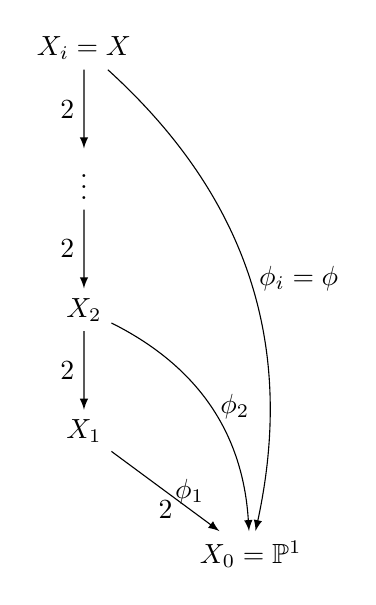
\begin{tikzpicture}[scale=0.3]
            \node at (0,0) (X0) {$X_0 = \PP^1$};
            \node [above left=of X0] (X1) {$X_1$};
            \node [above =of X1] (X2) {$X_2$};
            \node [above =of X2] (dots) {$\vdots$};
            \node [above =of dots] (Xr) {$X_i=X$};
            %\draw[<->] (X1) to node [above,rotate=-35] {$\sim$} node {} (X0);
            \draw[->] (X1) to node [below] {$2$} node [right] {$\phi_1$} (X0);
            \draw[->] (X2) to node [left] {$2$} node {} (X1);
            \draw[->, bend left] (X2) to node [below, right] {$\phi_2$} node {} (X0);
            \draw[->] (dots) to node [left] {$2$} node {} (X2);
            \draw[->] (Xr) to node [left] {$2$} node {} (dots);
            \draw[->, bend left] (Xr) to node [below, right] {$\phi_i=\phi$} node {} (X0);
            %\node at (8,0) (KX0) {$K(X_1) = K(\PP^1)$};
            %\node [above left=of KX0] (KX1) {$K(X_2)$};
            %\node [above =of KX1] (KX2) {$K(X_3)$};
            %\node [above =of KX2] (dots) {$\vdots$};
            %\node [above =of dots] (KXr) {$K(X_r)$};
            %%\draw[<->] (X1) to node [above,rotate=-35] {$\sim$} node {} (X0);
            %\draw[-] (KX1) to node [below] {$2$} node {} (KX0);
            %\draw[-] (KX2) to node [left] {$2$} node {} (KX1);
            %\draw[-, bend left] (KX2) to node [below, left] {} node {} (KX0);
            %\draw[-] (dots) to node [left] {$2$} node {} (KX2);
            %\draw[-] (KXr) to node [left] {$2$} node {} (dots);
            %\draw[-, bend left] (KXr) to node [below, left] {} node {} (KX0);
          \end{tikzpicture}
        \end{center}
        \caption{
          A $2$-group Belyi map $\phi$
          as a sequence of degree $2$ covers.
          For $j\in\{1,\dots,i\}$,
          $\phi$ factors through
          a degree $2^j$ Belyi map denoted $\phi_j$.
        }
        \label{fig:2groupfiltration}
      \end{figure}
      Let $\sigma_j$ be the permutation triple corresponding to
      $\phi_j$ in Figure \ref{fig:2groupfiltration}.
      Applying Algorithm \ref{alg:triples} to $\sigma_j$
      we obtain $\sigma_{j+1}$ as a lift of $\sigma_j$
      so that the permutation triple corresponding to $\phi$
      appears in $\mathscr{G}_{2^i}^\text{above}$.
      This shows that every $2$-group Belyi map
      of degree $2^i$ is represented by at least one node in
      $\mathscr{G}_{2^i}$.
      We now claim that every $2$-group Belyi map of degree $2^i$
      is represented by exactly one node in $\mathscr{G}_{2^i}$.
      % then show why only one in each iso class
      Since we are applying Algorithm \ref{alg:triples}
      to every permutation triple in $\mathscr{G}_{2^i}^\text{below}$,
      it is possible that in Step 2(a),
      the set of permutation triples in $\mathscr{G}_{2^i}^\text{above}$
      has simultaneously conjugate triples
      which arise when a degree $2^i$ Belyi map
      is a degree $2$ cover of more than one
      nonisomorphic Belyi map of degree $2^{i-1}$.
      In Step 2(b),
      we combine permutation triples in $\mathscr{G}_{2^i}^\text{above}$
      that are simultaneously conjugate by taking a single
      permutation triple to represent this isomorphism class
      of $2$-group Belyi map.
      Note that in Step 2(b)
      we never remove any edges in the graph
      $\mathscr{G}_{2^i}$.
      It follows from Step 2(b)
      that $\mathscr{G}_{2^i}^\text{above}$ has at most
      one node for each
      $2$-group Belyi map
      isomorphism class of degree $2^i$.
    \end{proof}
    \begin{theorem}\label{thm:isoclasses}
      The following table lists the number of isomorphism classes of
      $2$-group Belyi maps of degree $d$ for $d$ up to $256$.
      \[
        \begin{tabular}{|c||c|c|c|c|c|c|c|c|}
          \hline
          $d$ & $2$ & $4$ & $8$ & $16$ & $32$ & $64$ & $128$ & $256$\\
          \hline
          \# & $$ & $$ & $$ & $$ & $$ & $$ & $$ & $$\\
          \hline
        \end{tabular}
      \]
    \end{theorem}
    \begin{proof}
      Apply Algorithm \ref{alg:alltriples}.
      \mm{maybe go up to 512 or 1024 and include source code link to implementation}
    \end{proof}
    \begin{alg}\label{alg:allpassports}
      We use Algorithm \ref{alg:alltriples}
      to count the number of Passports of $2$-group Belyi maps
      of a given degree.
      \mm{todo}
    \end{alg}
    \begin{theorem}\label{thm:passports}
      The following table lists the number of passports of
      $2$-group Belyi maps of degree $d$ for $d$ up to $256$.
      \[
        \begin{tabular}{|c||c|c|c|c|c|c|c|c|}
          \hline
          $d$ & $2$ & $4$ & $8$ & $16$ & $32$ & $64$ & $128$ & $256$\\
          \hline
          \# passports & $3$ & $7$ & $16$ & $41$ & $96$ & $267$ & $834$ & $2893$\\
          \hline
        \end{tabular}
      \]
    \end{theorem}
    \begin{proof}
      Apply Algorithm \ref{alg:allpassports}.
    \end{proof}
  }
  \section{An algorithm to compute $2$-group Belyi curves and maps}{\label{sec:curvesandmaps}
    The algorithm we describe here is iterative.
    The degree $1$ case is discussed in Section \ref{sec:degree1}.
    We now set up some notation for the iteration.
    \begin{notation}\label{not:maps}
      First suppose
      we are given the following data:
      \begin{itemize}
        \item
          $X\subset\PP^n_K$ defined over a number field $K$
          with coordinates $x_0,\dots,x_n$
          cut out by the equations $\{h_i=0\}_i$ with $h_i\in K[x_0,\dots,x_n]$
        \item
          $\phi:X\to\PP^1$ a $2$-group Belyi map of degree $d=2^n$
          given by $\phi([x_0:\dots:x_n])=[x_0:x_1]$
          with monodromy group $G = \langle\sigma\rangle$
          (necessarily a $2$-group)
          with $\sigma$ a permutation triple corresponding to $\phi$
        \item
          For $s\in\{0,1,\infty\}$ and $\tau$ a cycle of $\sigma_s\in\sigma$,
          denote the ramification point above $s$ corresponding to
          $\tau$ by $Q_{s,\tau}$
        \item
          $Y\subset\AA^n_K$ the affine patch of $X$ with $x_0\neq 0$
          with coordinates $(y_1,\dots,y_n)$ where $y_i = x_i/x_0$
          cut out by the equations $\{g_i=0\}_i$ with $g_i\in K[y_1,\dots,y_n]$
          so that $\phi:Y\to\AA^1$ is given by $\phi(y_1,\dots,y_n) = y_1$
        \item
          $\wt{\sigma}$ as in the output of Algorithm \ref{alg:triples}
          applied to the input $\sigma$
      \end{itemize}
      Algorithm \ref{alg:lift} below
      describes how to lift the degree $d$ Belyi map $\phi$
      to a degree $2d$ Belyi map $\wt{\phi}$ with ramification prescribed by $\wt{\sigma}$
      (also see Figure \ref{fig:lift}).
    \end{notation}
    \begin{figure}[ht]
      \label{fig:lift}
      \[
        \begin{tikzcd}[ampersand replacement=\&]
          \widetilde{X}\arrow{dd}[swap]{\widetilde{\phi}}\arrow{dr}{\psi}\\
          % \widetilde{X}\arrow{dd}[swap]{\widetilde{\phi}}\arrow{dr}{\text{degree 2}}\\
          \&X\arrow{dl}{\phi}\\
          \PP^1
        \end{tikzcd}
      \]
      \caption{
      Algorithm \ref{alg:lift} describes how to construct $\wt{\phi}$
        corresponding to a permutation triple $\wt{\sigma}$
        from a given $2$-group Belyi map $\phi$.
        % In Algorithm \ref{alg:lift} we construct $\wt{\phi}$
        % from a given $2$-group Belyi map $\phi$.
      }
    \end{figure}
    \begin{lemma}\label{lem:1dim}
      Let $D$ be a degree $0$ divisor on $X$.
      Then $\ddim\LL(D) \leq 1$.
    \end{lemma}
    \begin{proof}
      Suppose $\ddeg D = 0$, and
      Let $f,g\in\LL(D)\setminus\{0\}$.
      Write $D=D_0-D_\infty$ with $D_0,D_\infty\geq 0$.
      Since $f,g\in\LL(D)$, we have
      $\ddiv f,\ddiv g\geq D_0-D_\infty$.
      In particular,
      $f/g\in K^\times$.
    \end{proof}
    \begin{definition}
      \label{def:ramificationful}
      Let $\phi\colon X\to\PP^1$ be a $2$-group Belyi map.
      Let $\ddiv\phi = D_0-D_\infty$
      and $\ddiv(\phi-1) = D_1 - D'_\infty$
      with $D_0, D_1, D_\infty, D'_\infty$ effective.
      For $s\in\{0,1,\infty\}$ let
      \[
        R_s \subseteq \supp D_s
      \]
      and $R\colonequals R_0+R_1+R_\infty$.
      Let $K$ be a number field
      containing the coordinates of
      all ramification points in $\supp R$
      and
      let
      \begin{equation}
        \label{eqn:ramificationful}
        M = (R+2\ZZ R)\cap\Div^0(X),
      \end{equation}
      and consider the map
      $M\to\Pic^0(X)(K)$.
      If this map has nontrivial kernel we say that
      $\phi$ is
      \defi{fully ramified for the ramification divisor $R$}.
    \end{definition}
    \begin{alg}\label{alg:lift}
      Let the notation be as described above in \ref{not:maps}.
      \newline
      \textbf{Input}:
      \begin{itemize}
        \item 
          $\phi:X\to\PP^1$ a $2$-group Belyi map
        \item
          $\wt{\sigma}$ a permutation triple which is a lift
          of $\sigma$ a permutation triple corresponding to $\phi$
        \item
          Suppose $\phi$ is fully ramified for
          $R$ in Step \ref{prescribedramification}
      \end{itemize}
      \textbf{Output}: A model over a number field $K$ for the Belyi map
      $\wt{\phi}:\wt{X}\to\PP^1$
      with monodromy $\wt{\sigma}$.
      \begin{enumerate}
        \item
          \label{prescribedramification}
          Let $R$ be the empty set of points on $X$.
          For each $s\in\{0,1,\infty\}$,
          If the order of $\sigma_s$ is strictly less than the order of $\wt{\sigma}_s$,
          then append the ramification points
          $\{Q_{s,\tau}\}_{\tau\in\sigma_s}$
          (the ramification points on $X$ above $s$ corresponding to the cycles of $\sigma_s$)
          to $R$.
        \item
          Let $K$ be a number field containing all coordinates of
          points in $R$
          (a subset of the ramification points of $\phi$).
        % \item
        %   Let $D = \sum_{P}n_PP$ be a degree $0$ divisor on $X$ 
        %   with $n_P$ odd for every $P\in R$
        %   and $n_P = 0$ for $P\not\in R$.
        %   \mm{class group and base field}
        \item
          Let $M = (R+2\ZZ R)\cap\Div^0(X)$.
        \item
          \label{ramificationfulloop}
          For each $D\in M$ do the following:
          \begin{itemize}
            \item
              Compute the Riemann-Roch space $\LL(D)$.
            \item
              If $\dim\LL(D) = 1$, then
              compute $f\in K(X)^\times$
              corresponding to a generator
              of $\LL(D)$
              exit the loop
              and go to Step \ref{wefoundafunction}.
            \item
              If $\dim\LL(D) = 0$,
              then continue this loop
              with another choice of $D$.
          \end{itemize}
        \item
          \label{wefoundafunction}
          Write $f=a/b$ with $a,b\in K[y_1,\dots,y_n]$ and construct the ideal
          \[
            \wt{I}\colonequals\langle g_1,\dots,g_k, by_{n+1}^2-a\rangle
          \]
          in $K[y_1,\dots,y_n,y_{n+1}]$.
        \item
          \label{saturate}
          Saturate $\wt{I}$ at $\langle b\rangle$ and denote this ideal by $\sat(\wt{I})$.
        \item
          Let $\wt{X}$ be the curve corresponding to $\sat(\wt{I})$ and
          $\wt{\phi}$ the map $(y_1,\dots,y_{n+1})\mapsto y_1$.
      \end{enumerate}
    \end{alg}
    \begin{proof}[Proof of correctness]
      By Algorithm \ref{alg:triples},
      there exists a $2$-group Belyi map $\wt{\phi}:\wt{X}\to\PP^1$
      with ramification according to $\wt{\sigma}$.
      Since $\wt{\phi}$ is Galois,
      the ramification behavior above each $s\in\{0,1,\infty\}$
      is constant
      (i.e. for a fixed $s$, all $Q_{s,\tau}$ are either unramified or
      ramified to order $2$).
      This ensures that the set $R$ constructed in Step $1$
      is precisely the set of ramification values of $\psi$
      (in Figure \ref{fig:lift}).
      Now that we have the ramification points,
      we can construct the new Belyi map and curve
      by extracting a square root in the function field.
      More precisely,
      again by Algorithm \ref{alg:triples},
      there exists $\wt{X}$ and a number field $K$
      with $K(\wt{X}) = K(X,\sqrt{f})$
      where $f\in K(X)^\times/K(X)^{\times 2}$
      and
      \begin{equation}\label{eqn:classgroup}
        \ddiv f= \sum_{Q_{s,\tau}\in R} Q_{s,\tau}+2D_\epsilon
        \in\frac{\Div^0(X)}{2\Div^0(X)}
      \end{equation}
      Since $\phi$ is fully ramified for $R$,
      there is a $D\in M$ such that
      $f\in\LL(D)$
      will be obtained in Step \ref{ramificationfulloop}.
      In Step \ref{wefoundafunction}
      we start with the ideal of $X$
      and add a new equation (using an extra variable)
      corresponding to extracting the square root of $f$.
      This is our candidate ideal for $\wt{X}$,
      but this process may introduce extra components.
      To eliminate these components, we saturate the ideal
      in Step \ref{saturate}.
      By construction,
      the projection map to the first (affine)
      coordinate
      is the desired Belyi map
      with Belyi curve $\wt{X}$.
    \end{proof}
    \begin{remark}
      \label{rmk:fullyramifiedinpractice}
      The condition that $\phi$
      is fully ramified is required
      to avoid a potentially infinite loop in
      Step \ref{ramificationfulloop}.
      Testing this condition is only implemented over
      a finite field,
      so in practice we simply search for candidate divisors
      in $M$ without testing if $\phi$ is fully ramified.
      This appears to work well in practice,
      and has been used to carry out the explicit computations
      in Section \ref{sec:computations}.
    \end{remark}
    \begin{remark}
      \label{rmk:basefield}
      Another important aspect of this process is the choice of $K$.
      In Algorithm \ref{alg:lift},
      we try to keep the degree of $K$ as small as possible.
      Adjoining all coordinates of ramification points
      can lead to high degree extensions
      which are not feasible in practice.
      We choose to obtain the Belyi curve
      over a subfield when possible.
    \end{remark}
  }
  \section{Running time analysis}{\label{sec:runtime}
  }
  \section{Explicit computations}{\label{sec:computations}
    \mm{link to database, code, and some tables}
  }
} 
\chapter{Classifying low genus and hyperelliptic $2$-group Belyi maps}{\label{chapter:classify}
  In this chapter we organize some results on $2$-group Belyi maps
  with low genus.
  The conditions that need to be satisfied for a general Belyi map
  to be a $2$-group Belyi map are quite stringent.
  This allows us to give a clear picture of the story
  in these special cases.
  \section{Remarks on Galois Belyi maps}{\label{sec:galoisbelyimaps}
    We summarize some of the results on Galois Belyi maps
    that we use for $2$-group Belyi maps.
    A great deal is known about Galois Belyi maps (regular dessins) in general
    (see \mm{TODO: sources}).
    \begin{lemma}\label{lem:regular}
      Let $\sigma$ be a degree $d$ permutation triple corresponding to
      $\phi\colon X\to\PP^1$ a Galois Belyi map with monodromy group $G$
      and
      $m_s$ be the order of $\sigma_s$ for $s\in\{0,1,\infty\}$.
      Then $\sigma_s$ consists of $d/m_s$ many $m_s$-cycles.
      In particular,
      for a $2$-group Belyi map,
      $m_s$ and $\#G$ are powers of $2$.
    \end{lemma}
    \begin{proof}
    \end{proof}
    In light of Lemma \ref{lem:regular},
    we get a refined version of Riemann-Hurwitz for Galois Belyi maps.
    \begin{prop}\label{prop:riemannhurwitzgalois}
      Let $\sigma$ be a degree $d$ permutation triple corresponding to
      $\phi\colon X\to\PP^1$ a Galois Belyi map with monodromy group $G$.
      Let $a,b,c$ be the orders of $\sigma_0,\sigma_1,\sigma_\infty$
      respectively.
      Then
      \begin{equation}\label{eqn:riemannhurwitzgalois}
        g(X) = 1+\frac{\#G}{2}\left(1-\frac{1}{a}-\frac{1}{b}-\frac{1}{c}\right).
      \end{equation}
    \end{prop}
    \begin{proof}
    \end{proof}
  }
  \section{Genus $0$}{\label{sec:genuszero}
    Let $\phi:X\to\PP^1$ be a $2$-group Belyi map where $X$ has genus $0$.
    Proposition \ref{prop:riemannhurwitzgalois} immediately restricts the
    possibilities for ramification indices.
    \begin{prop}\label{prop:genuszeroramification}
      A $2$-group Belyi map of genus $0$ with monodromy group $G$
      has the following possibilities for ramification indices:
      \begin{itemize}
        \item degenerate: $(1,\#G, \#G)$, $(\#G, 1, \#G)$, $(\#G, \#G, 1)$
        \item
          dihedral:
          $\left(\frac{\#G}{2}, 2, 2\right)$,
          $\left(2, \frac{\#G}{2}, 2\right)$,
          $\left(2, 2, \frac{\#G}{2}\right)$
      \end{itemize}
    \end{prop}
    \begin{proof}
      Let $a,b,c$ be the ramification indices of the Belyi map.
      Then by Lemma \ref{lem:regular},
      $a,b,c,\#G$ are all positive powers of $2$.
      Without loss of generality we may assume $a\le b\le c$.
      The proof is by cases.
      For $g(X)=0$, Proposition \ref{prop:riemannhurwitzgalois}
      yields
      \begin{equation}\label{eqn:riemannhurwitzgenuszero}
        \frac{\#G}{2}\left(1-\frac{1}{a}-\frac{1}{b}-\frac{1}{c}\right) = -1.
      \end{equation}
      \begin{itemize}
        \item[\underline{$a=1$}:]
          If $a=1$, then
          Equation \ref{eqn:riemannhurwitzgenuszero} becomes
          $\frac{1}{b}+\frac{1}{c}=\frac{2}{\#G}$.
          \begin{itemize}
            \item[\underline{$b=1$}:]
              If $a=b=1$, then
              Equation \ref{eqn:riemannhurwitzgenuszero}
              implies $a=b=c=\#G=1$.
            \item[\underline{$b\ge 2$}:]
              If $a=1$ and $b\geq 2$,
              then we can let $b=2^m$ and $c=2^n$ with $m\le n$.
              In this case
              Equation \ref{eqn:riemannhurwitzgenuszero} becomes
              \[
                \frac{1}{2^m}+\frac{1}{2^n} = \frac{2}{\#G}
                \implies
                \#G\left(2^{n-m}+1\right) = 2^{n+1}.
              \]
              Since $\#G$ is a power of $2$, we must have
              $2^{n-m}+1\in\{1,2\}$ which only occurs when $m=n$.
              Therefore $m=n$ which implies $b=c=\#G$.
          \end{itemize}
        \item[\underline{$a=2$}:]
          If $a=2$, then
          Equation \ref{eqn:riemannhurwitzgenuszero} becomes
          \[
            \frac{2}{\#G} = \frac{1}{b}+\frac{1}{c}-\frac{1}{2}.
          \]
          \begin{itemize}
            \item[\underline{$b=2$}:]
              If $a=2$ and $b=2$, then
              Equation \ref{eqn:riemannhurwitzgenuszero} implies
              $c=\frac{\#G}{2}$.
            \item[\underline{$b\ge 4$}:]
              If $a=2$ and $b,c\geq 4$, then
              Equation \ref{eqn:riemannhurwitzgenuszero} implies
              \[
                \frac{2}{\#G} = \frac{1}{b}+\frac{1}{c}-\frac{1}{2}
                \implies
                \frac{2}{\#G}\le 0
              \]
              which cannot occur.
          \end{itemize}
        \item[\underline{$a\geq 4$}:]
          If $a,b,c\geq 4$, then
          Equation \ref{eqn:riemannhurwitzgenuszero} becomes
          \[
            \frac{2}{\#G} = \frac{1}{b}+\frac{1}{c} - \left(1-\frac{1}{a}\right).
          \]
          But
          $\left(1-\frac{1}{a}\right)\ge\frac{3}{4}$
          and
          $\frac{1}{b}+\frac{1}{c}\le\frac{1}{2}$
          imply that
          $\frac{2}{\#G}<0$
          which cannot occur.
      \end{itemize}
      In summary there are $2$ possibilities:
      \begin{itemize}
        \item $a=1$ and $b=c=\#G$
        \item $a=2$, $b=2$, and $c=\frac{\#G}{2}$
      \end{itemize}
      By reordering the ramification indices
      we obtain the possibilities in Proposition \ref{prop:genuszeroramification}.
    \end{proof}
    In particular,
    from
    Proposition \ref{prop:genuszeroramification}
    we see that all genus $0$ $2$-group Belyi maps
    are degenerate or spherical dihedral.
    The explicit maps in these cases are well understood
    \mm{TODO: cite}\cite{turkishbelyithesis}.
    We summarize with Proposition \ref{prop:turkishbelyithesis}.
    \begin{prop}\label{prop:turkishbelyithesis}
      Every possible ramification type in
      Proposition \ref{prop:genuszeroramification}
      corresponds to exactly one Belyi map up to isomorphism.
      Moreover, the equations for these maps have simple formulas
      given below.
      In the formulas below,
      we use the notation from Proposition \ref{prop:genuszeroramification}
      for ramification types and write a Belyi map
      $\phi:\PP^1\to\PP^1$ with monodromy $G$
      as a rational function in the coordinate $x$
      on an affine patch of the domain of $\phi$.
      \begin{itemize}
        \item
          $(1,1,1)$
          \[
            \phi(x) = x
          \]
        \item
          $(1,\#G, \#G)$, $\#G\ge 2$
          \[
            \phi(x) = 1-x^{\#G}
          \]
        \item
          $(\#G, 1, \#G)$, $\#G\ge 2$
          \[
            \phi(x) = x^{\#G}
          \]
        \item
          $(\#G, \#G, 1)$, $\#G\ge 2$
          \[
            \phi(x) = \frac{x^{\#G}}{x^{\#G}-1}
          \]
        \item
          $(2, 2, 2)$, $\#G = 2$
          \[
            \phi(x) = -\left(\frac{x(x-1)}{x-\frac{1}{2}}\right)^2
          \]
        \item
          $(2, 2, \frac{\#G}{2})$, $\#G\ge 4$
          \[
            \phi(x) = -\frac{1}{4}\left(x^{\#G/2}+\frac{1}{x^{\#G/2}}\right)
            +\frac{1}{2}
          \]
        \item
          $(2, \frac{\#G}{2}, 2)$, $\#G\ge 4$
          \[
            \phi(x) = 1-\frac{1}{1-\left(-\frac{1}{4}\left(x^{\#G/2}+\frac{1}{x^{\#G/2}}\right)
            +\frac{1}{2}\right)}
          \]
        \item
          $(\frac{\#G}{2}, 2, 2)$, $\#G\ge 4$
          \[
            \phi(x) = \frac{1}{-\frac{1}{4}\left(x^{\#G/2}+\frac{1}{x^{\#G/2}}\right)
            +\frac{1}{2}}
          \]
      \end{itemize}
    \end{prop}
    \begin{proof}
      We first address the correctness of the equations.
      For the ramification triples containing $1$,
      the equations are all lax isomorphic to one of the form
      \begin{equation}\label{eqn:squaringmap}
        \phi(x) = x^{\#G}
      \end{equation}
      for the ramification triple
      $(\#G, 1, \#G)$.
      The rational function $\phi$ in Equation \ref{eqn:squaringmap}
      has a root of multiplicity $\#G$ at $0$,
      a pole of multiplicity $\#G$ at $\infty$,
      and $\#G$ unique preimages above $1$.
      The Belyi maps for ramification triples
      $(1,\#G, \#G)$ and $(\#G, \#G, 1)$
      are lax isomorphic to $\phi$ in Equation \ref{eqn:squaringmap}
      and similarly have the correct ramification of this
      degenerate Belyi map.
      \par
      For the other ramification triples, we focus on
      the triple $(2,2,\frac{\#G}{2})$.
      The equation for this map is a modification
      (pointed out to me by Sam Schiavone)
      of the dihedral Belyi map
      \begin{equation}\label{eqn:dihedral}
        \phi(x) = x^d+\frac{1}{x^d}
      \end{equation}
      in \cite[Example 5.1.2]{turkishbelyithesis}.
      The other dihedral maps are then lax isomorphic to
      (the modification of) the map in Equation \ref{eqn:dihedral}.
      \par
      To show that there is at most one Belyi map in each of the above cases,
      we refer to Algorithm \ref{alg:triples}.
      \mm{todo}
    \end{proof}
  }
  \section{Genus $1$}{\label{sec:genusone}
    Let $\phi\colon X\to\PP^1$ be a $2$-group Belyi map
    where $X$ has genus $1$.
    Let $(a,b,c)$ be the ramification indices of $\phi$
    with $a\leq b\leq c$.
    From Proposition \ref{prop:riemannhurwitzgalois},
    we have that
    \begin{equation}\label{eqn:genusoneramification}
      % \frac{\#G}{2}\left(1-\frac{1}{a}-\frac{1}{b}-\frac{1}{c}\right) = 0
      % \implies
      % \left(1-\frac{1}{a}-\frac{1}{b}-\frac{1}{c}\right) = 0.
      \frac{1}{a}+\frac{1}{b}+\frac{1}{c} = 0.
    \end{equation}
    Since $a,b,c$ are powers of $2$,
    the only solution to
    Equation \ref{eqn:genusoneramification}
    is $a=2$ and $b=c=4$.
    We summarize this discussion in
    Proposition \ref{prop:genusoneramification}.
    \begin{prop}\label{prop:genusoneramification}
      The only possible ramification indices for
      a $2$-group Belyi map of genus $1$
      are $(2,4,4)$, $(4,2,4)$, or $(4,4,2)$.
    \end{prop}
    As was the case in genus $0$,
    all ramification triples in
    Proposition \ref{prop:genusoneramification}
    have corresponding Belyi maps.
    However, as we see in
    Proposition \ref{prop:genusonemaps},
    these genus $1$ Belyi maps occur in infinite families.
    \begin{prop}\label{prop:genusonemaps}
      Let $(a,b,c)$ be a ramification triple in
      Proposition \ref{prop:genusoneramification}
      and let $d = 2^m$ for $m\in\ZZ_{\geq 2}$.
      Then there exists exactly one
      degree $d$ $2$-group Belyi map up to isomorpism
      with ramification $(a,b,c)$.
      Moreover, the equations for these maps have simple formulas
      which are described below.
      In these equations let $E$ be the elliptic curve
      with $j$-invariant $1728$ given by the Weierstrass equation
      \[
        E\colon y^2 = x^3+x.
      \]
      Every degree $4$ Belyi map below is of the form
      $\phi\colon E\to\PP^1$ where $\phi$
      (written as an element of the function field of $E$)
      is one of the following:
      \begin{align}\label{eqn:d4g1}
        \begin{split}
          \phi_{(2,4,4)} &= \frac{x^2+1}{x^2}\\
          \phi_{(4,2,4)} &= \phi_{(2,4,4)} - 1=-\frac{1}{x^2}\\
          \phi_{(4,4,2)} &= \frac{1}{\phi_{(2,4,4)}} = \frac{x^2}{x^2+1}
        \end{split}
      \end{align}
      Every degree $d$ Belyi map
      for $d\geq 8$ is of the form
      \[
        E\stackrel{\psi}{\to}E\stackrel{\phi}{\to}\PP^1
      \]
      where $\phi$ is a degree $4$ genus $1$ Belyi map
      and $\psi$ is degree $d/4$ isogeny of $E$.
      Moreover,
      if we let $\alpha\colon E\to E$ be defined by
      \begin{equation}\label{eqn:alpha}
        (x,y)\mapsto
        \left(
          (1+\sqrt{-1})^{-2}\left(x+\frac{1}{x}\right),
          (1+\sqrt{-1})^{-3}y\left(1-\frac{1}{x^2}\right)
        \right)
      \end{equation}
      then $\psi$ is the map $\alpha$ composed with itself
      $d/8$ times.
    \end{prop}
    \begin{proof}
      For a proof that these are the only such $2$-group Belyi maps
      we used \cite[Lemma 3.5]{triangles}.
      This can also be seen from Algorithm \ref{alg:alltriples}.
      The degree $4$ Belyi maps are all lax isomorphic
      to the degree $4$ genus $1$ Belyi map with
      ramification indices $(4,4,2)$ in
      \cite{belyidb}.
      For degree $d$ with $d\geq 8$
      let $\phi$ be one of the degree $4$ maps in
      Equation \ref{eqn:d4g1}.
      We then precompose
      $\phi$
      with $\alpha\cdots\alpha$ ($d/8$ times)
      where $\alpha$ is the
      degree $2$ endomorphism of $E$
      found in
      \cite[Proposition 2.3.1]{advancedsilverman}.
      Since isogenies are unramified
      in characteristic $0$
      (see \cite[Chapter III, Theorem 4.10]{silverman})
      the composition $\phi\alpha^{d/8}$
      is a degree $d$ Belyi map with the same ramification type as $\phi$.
    \end{proof}
  }
  \section{Hyperelliptic}{\label{sec:hyperelliptic}
    \begin{definition}\label{def:hyperelliptic}
      Let $\phi\colon X\to\PP^1$ be a Belyi map
      of genus $\geq 2$.
      We say a Belyi map $\phi$ is \defi{hyperelliptic}
      if $X$ is a hyperelliptic curve.
      A hyperelliptic curve $X$ over $\CC$
      is defined by having
      an element $\iota\in\Aut(X)$
      such that
      the quotient map
      $X\to X/\langle\iota\rangle$
      is a degree $2$ map to $\PP^1$.
      This element $\iota$ is known as the
      \defi{hyperelliptic involution}.
    \end{definition}
    Let $\phi\colon X\to\PP^1$ be a hyperelliptic
    $2$-group Belyi map with monodromy group
    $H\leq G\colonequals\Aut(X)$,
    and hyperelliptic involution $\iota\in\Aut(X)$.
    \begin{lemma}\label{lem:hypinvolutioncentral}
      % $G\leq\Aut(X)$ and $\iota$ is central in $G$.
      $\langle\iota\rangle\trianglelefteq\Aut(X)$
    \end{lemma}
    \begin{proof}
    \end{proof}
    \begin{definition}\label{def:reducedautomorphismgroup}
      The
      \defi{reduced automorphism group} of $X$
      is the quotient group
      $G_{\rred}\colonequals G/\langle\iota\rangle$.
    \end{definition}
    % \begin{lemma}\label{lem:normalsubgroup}
    %   $H\trianglelefteq\Aut(X)$.
    % \end{lemma}
    From Lemma \ref{lem:hypinvolutioncentral}
    and the Galois condition on $\phi$,
    we obtain the diagram in Figure \ref{fig:hyperellipticbelyi}.
    \begin{figure}[ht]
      \[
        \begin{tikzcd}
          &X\arrow[swap, Rightarrow]{dl}{\phi}\arrow[Rightarrow]{dr}{\langle\iota\rangle}
          \arrow[Rightarrow]{dd}{\psi}\\
          \PP^1\simeq X/H\arrow{dr}&&\PP^1\simeq X/\langle\iota\rangle\arrow[Rightarrow]{dl}{G/\langle\iota\rangle}\\
                         &\PP^1\simeq X/G
        \end{tikzcd}
      \]
      \caption{Galois theory for a hyperelliptic Belyi map}
      \label{fig:hyperellipticbelyi}
    \end{figure}
    \begin{prop}\label{prop:liftbelyi}
      Let $\phi$ and $\psi$ be the maps shown in
      Figure \ref{fig:hyperellipticbelyi}.
      If $\phi$ is a Belyi map,
      then $\psi$ is a Belyi map.
    \end{prop}
    \begin{proof}
      By Theorem \ref{thm:bigbijection},
      $\phi$ corresponds to
      a normal inclusion of triangle groups
      $
        \Delta_1\trianglelefteq\Delta_H
      $
      and the map $X / H \to X / G$
      corresponds to an inclusion of Fuchsian groups
      \begin{equation}\label{eqn:fuchsianinclusion}
        \Delta_H\leq\Gamma.
      \end{equation}
      By a result in \cite[Page 36]{singerman},
      the inclusion of a triangle group $\Delta_H$ in
      a Fuchsian group $\Gamma$
      as in Equation \ref{eqn:fuchsianinclusion}
      implies that $\Gamma$ is a triangle group
      which we denote $\Delta_G$.
      Now we have the
      (normal by Lemma \ref{lem:hypinvolutioncentral})
      inclusion
      $\Delta_1\trianglelefteq\Delta_G$
      which (again by Theorem \ref{thm:bigbijection})
      implies that $\psi$ is a Belyi map.
    \end{proof}
    Proposition \ref{prop:liftbelyi}
    reduces the classification of these hyperelliptic $2$-group Belyi maps
    to the situation on the right side of the diagram in
    Figure \ref{fig:hyperellipticbelyi}.
    The possibilities for $G_{\rred}$
    in this setting are known
    (see \cite[\S 1.1]{dolgachev}).
    Moreover, since $G$ is a
    $2$-group (\mm{$G$ only contains a $2$-group\ldots}),
    the only possibilities for $G_{\rred}$
    are cyclic or dihedral of order $\#G / 2$.
    $G$ is then an extension of $G_{\rred}$
    by $\iota$
    (an element of order $2$ generating a normal subgroup of $G$).
    Such groups are classified in
    \cite{hyperelliptic} which we summarize in the
    following theorem.
    \begin{theorem}
      \label{thm:hyperelliptic}
      Let $G$ be the full automorphism group of a
      $2$-group Belyi curve.
      Let $\#G_{\rred} = 2^n$.
      Then $G$ is isomorphic to one of the following groups:
      \begin{itemize}
        \item
          $\ZZ/2^{n+1}\ZZ$
        \item
          $\ZZ / 2^n\ZZ\times\ZZ / 2\ZZ$
        \item
          $D_{2^{n+1}}$
        \item
          $D_{2^n}\times\ZZ / 2\ZZ$
      \end{itemize}
      where $D_m$ denotes the dihedral group of order $m$.
    \end{theorem}
    \begin{proof}
      \cite[Theorem 2.1]{hyperelliptic}.
    \end{proof}
    \mm{
      you get a genus zero phi0 : Belyi map
      PP1 $\to$ PP1 and the degree 2 map on top must be ramified,
      corresponding to the hyperelliptic involution, can only be ramified
      along the preimages of ramification points of phi0, and in a
      group-invariant way, so that should really give you the equations as
      well.
    }
    \newline
    \mm{
      maybe write down explicit maps for g=2,3
    }
      %   \begin{theorem}\label{thm:hyperelliptic}
      %     Let $\phi:X\to\PP^1$ be a hyperelliptic $2$-group Belyi map
      %     with monodromy group $G$.
      %     Let $\iota$ denote the hyperelliptic involution in $\Aut(X)$.
      %     Then $\overline{G}\colonequals G/\langle\iota\rangle$
      %     is a subgroup of $\Aut(\PP^1)\cong\PGL_2(\CC)$.
      %     (see Figure \ref{fig:hyperelliptic}).
      %     In particular,
      %     $\overline{G}$ is either cyclic, dihedral, or exceptional.
      %     \begin{figure}[ht]
      %       \[
      %         \begin{tikzcd}[ampersand replacement=\&]
      %           X\arrow{dd}[swap]{G}\arrow{dr}{\langle\iota\rangle}\\
      %           \&\PP^1\arrow{dl}{G/\langle\iota\rangle}\\
      %           \PP^1
      %         \end{tikzcd}
      %       \]
      %       \caption{
      %         A hyperelliptic $2$-group Belyi map
      %         with monodromy group $G$
      %         factors through a degree $2$ map to $\PP^1$
      %         and an automorphism of $\PP^1$.
      %       }
      %       \label{fig:hyperelliptic}
      %     \end{figure}
      %   \end{theorem}
  }
    % We start Section \ref{sec:classification} by giving a complete description of the geometry type
    % (see Definition \ref{def:geometrytype}) of a
    % $2$-group Belyi map in Proposition \ref{prop:geometrytype}
    % and finish Section \ref{sec:classification}
    % with a classification of hyperelliptic
    % $2$-group Belyi maps in Theorem \ref{thm:hyperelliptic}.
    % \begin{prop}\label{prop:geometrytype}
    %   Let $\phi:X\to\PP^1$ be a $2$-group Belyi map
    %   corresponding to a permutation triple $\sigma$
    %   with $(a,b,c)$ the triple of orders of permutations in $\sigma$.
    %   Then the geometry type of $\phi$ is determined by $(a,b,c)$
    %   and is one of the following:
    %   \begin{enumerate}
    %     \item[(degenerate)]
    %       $\phi$ is degenerate if $1\in(a,b,c)$.
    %     \item[(spherical)]
    %       $\phi$ is spherical if $(a,b,c)$ is of the form
    %       $(2,2,c)$, $(2,b,2)$, or $(a,2,2)$.
    %     \item[(Euclidean)]
    %       $\phi$ is Euclidean if $(a,b,c)$ is of the form
    %       $(2,4,4)$, $(4,2,4)$, or $(4,4,2)$.
    %     \item[(hyperbolic)]
    %       $\phi$ is hyperbolic (with genus at least $2$) in all other cases.
    %   \end{enumerate}
    % \end{prop}
    % \begin{proof}
    % \end{proof}
    % \subsection{Classifying spherical $2$-group Belyi maps}{\label{subsec:elliptic}}{
    % }
    % \subsection{Classifying genus $1$ $2$-group Belyi maps}{\label{subsec:elliptic}}{
    % }
    % \subsection{Classifying hyperelliptic $2$-group Belyi maps}{\label{subsec:hyperelliptic}}{
      % \begin{definition}
      %   Let $K$ be a number field with algebraic closure $\overline{K}$.
      %   Let $X$ be an irreducible smooth projective curve over $K$.
      %   $X$ is \defi{hyperelliptic} if there exists a degree $2$ map
      %   $\iota:X\to\PP^1$ (defined over $\overline{K}$).
      %   The degree $2$ map $\iota$ is called the
      %   \defi{hyperelliptic involution}.
      % \end{definition}
    %   \begin{definition}
    %     A \defi{hyperelliptic Belyi map} is a Belyi map $\phi:X\to\PP^1$
    %     where $X$ is a hyperelliptic curve.
    %   \end{definition}
      %   \begin{lemma}\label{lem:hypinvolutioncentral}
      %     Let $\phi:X\to\PP^1$ be a hyperelliptic $2$-group Belyi map
      %     with monodromy group $G$.
      %     Let $\iota$ denote the hyperelliptic involution in $\Aut(X)$.
      %     Then
      %     $G\leq\Aut(X)$ and $\iota$ is central in $G$.
      %   \end{lemma}
    %   \begin{proof}
    %   \end{proof}
      %   \begin{theorem}\label{thm:hyperelliptic}
      %     Let $\phi:X\to\PP^1$ be a hyperelliptic $2$-group Belyi map
      %     with monodromy group $G$.
      %     Let $\iota$ denote the hyperelliptic involution in $\Aut(X)$.
      %     Then $\overline{G}\colonequals G/\langle\iota\rangle$
      %     is a subgroup of $\Aut(\PP^1)\cong\PGL_2(\CC)$.
      %     (see Figure \ref{fig:hyperelliptic}).
      %     In particular,
      %     $\overline{G}$ is either cyclic, dihedral, or exceptional.
      %     \begin{figure}[ht]
      %       \[
      %         \begin{tikzcd}[ampersand replacement=\&]
      %           X\arrow{dd}[swap]{G}\arrow{dr}{\langle\iota\rangle}\\
      %           \&\PP^1\arrow{dl}{G/\langle\iota\rangle}\\
      %           \PP^1
      %         \end{tikzcd}
      %       \]
      %       \caption{
      %         A hyperelliptic $2$-group Belyi map
      %         with monodromy group $G$
      %         factors through a degree $2$ map to $\PP^1$
      %         and an automorphism of $\PP^1$.
      %       }
      %       \label{fig:hyperelliptic}
      %     \end{figure}
      %   \end{theorem}
    %   \begin{proof}
    %   \end{proof}
    % }
}
\chapter{Fields of definition of $2$-group Belyi maps}{\label{chapter:fieldsofdefinition}
  Using data from Chapter \ref{chapter:database},
  we formulate a conjecture about the possible fields of definition of
  $2$-group Belyi maps.
  Recall Section
  \ref{subsec:fieldsofmodulifieldsofdefinition}
  on fields of moduli and fields of definition
  and
  Recall Section \ref{subsec:passports} on passports.
  % \section{Fields of moduli}{\label{sec:fieldsofmoduli}}{
  %   Recall the action of $G_\QQ$ on the set of Belyi maps
  %   described in Proposition \ref{prop:galoisaction}.
  %   For a fixed Belyi map,
  %   we can simplify matters as described in the following definition.
  %   \begin{definition}\label{def:fieldofmoduli}
  %     The \defi{field of moduli} of a Belyi map
  %     $\phi:X\to\PP^1$ is the fixed field
  %     \[
  %       \{\tau\in G_\QQ : \phi^\tau\cong\phi\}.
  %     \]
  %   \end{definition}
  %   Definition \ref{def:fieldofmoduli} allows us to study
  %   a more manageable finite extension.
  %   Moreover, passports (recall Definition \ref{def:passport})
  %   allow us to bound the degree of the field of moduli.
  %   \begin{theorem}\label{thm:fieldofmoduli}
  %     Let $\phi:X\to\PP^1$ be a Belyi map
  %     with passport $\mathcal{P}$.
  %     Then the degree of the field of moduli of $\phi$
  %     is bounded by the size of $\mathcal{P}$.
  %   \end{theorem}
  %   \begin{proof}
  %     % proof in JVSijsling
  %   \end{proof}
  % }
  \section{Refined passports}{\label{sec:refined}}{
    \begin{definition}\label{def:refined}
      A \defi{refined passport} $\mathcal{P}$ consists of the data
      $(g,G,C)$
      where $g\geq 0$ is an integer,
      $G\leq S_d$ is a transitive subgroup,
      and $C = (C_0,C_1,C_\infty)$
      is a triple of conjugacy classes of $G$.
    \end{definition}
    \mm{some exposition about refined passports}
    For a refined passport $\mathcal{P}$ consider the set
    \[
      \Sigma_\mathcal{P} =
      \{(\sigma_0,\sigma_1,\sigma_\infty)\in C_0\times C_1\times C_\infty : \sigma_\infty\sigma_1\sigma_0=1,\text{ and } \langle\sigma\rangle=G\}/\sim
    \]
    where $(\sigma_0,\sigma_1,\sigma_\infty)\sim(\sigma_0', \sigma_1', \sigma_\infty')$
    if and only if there exists $\alpha\in\Aut(G)$ with
    $\alpha(\sigma_s) = \sigma_s'$ for $s\in\{0,1,\infty\}$.
  }
  \section{A refined conjecture}{\label{sec:conjecture}}{
    \begin{conj}
      Let $\mathcal{P} = (g,G,C)$
      be a refined passport with
      $G=\Mon(\phi)$ for some $2$-group Belyi map $\phi$.
      Then $\#\Sigma_\mathcal{P} = 0\text{ or }1$.
    \end{conj}
    \begin{proof}
      \mm{computational evidence, true in easy cases}
    \end{proof}
    \begin{corr}
      Every $2$-group Belyi map is defined over a cyclotomic field
      $\QQ(\zeta_{2^m})$ for some $m$.
    \end{corr}
    \begin{proof}
      \mm{
        The group $\Gal(\QQal/\QQab)$ acts on the refined passport
      }
    \end{proof}
  }
}
\chapter{Gross's conjecture for $p=2$}{\label{chapter:grossconjecture}
  We begin this chapter with Theorem \ref{thm:beckmann} which provides
  the arithmetic motivation to study $2$-group Belyi maps.
  We then detail past results on Gross's conjecture in Section
  \ref{sec:grossconjecturepast}
  and finish with some discussion on $2$-group Belyi maps
  in relation to the $p=2$ case of Gross's conjecture.
  \section{Beckmann's theorem}{\label{sec:beckmann}
    In this Section we state Beckmann's theorem
    for Belyi maps over $\CC$
    from
    $1989$ which can be found in \cite{beckmann}.
    We then adapt Theorem \ref{thm:beckmann}
    to our particular situation in
    Corollary \ref{cor:beckmann}.
    \begin{theorem}\label{thm:beckmann}
      Let $\phi:X\to\PP^1$ be a Belyi map with
      monodromy group $G$
      and suppose $p$ does not divide $\# G$.
      Then there exists a number field $M$
      with the following properties:
      \begin{itemize}
        \item
          $p$ is unramified in $M$
        \item
          the Belyi map $\phi$ is defined over $M$
        \item
          the Belyi curve $X$ is defined over $M$
        \item
          $X$ has good reduction at all primes $\mathfrak{p}$
          of $M$ above $p$
      \end{itemize}
    \end{theorem}
    \begin{proof}
      \cite{beckmann}
    \end{proof}
    \begin{corr}\label{cor:beckmann}
      Let $\phi:X\to\PP^1$ be a $2$-group Belyi map.
      Then there exists a smooth projective model for $X$
      with good reduction away from $p=2$.
    \end{corr}
    \begin{proof}
    \end{proof}
  }
  \section{Past results on Gross's conjecture}{\label{sec:grossconjecturepast}
  }
  \section{A nonsolvable Galois number field ramified only at $2$}{\label{sec:numberfieldramifiedat2}
  }
}


%%%%%%%%%%%%%%%%%%%%%%%%%%%%%%%%%%%%%%%%%%%%%%%%%%
%Backend of thesis (references and the like)
%%%%%%%%%%%%%%%%%%%%%%%%%%%%%%%%%%%%%%%%%%%%%%%%%%
\backmatter

%Add your bibliography filename and uncomment these lines
\bibliographystyle{amsplain}
\addcontentsline{toc}{chapter}{References}
\bibliography{references}

%Uncomment if you want an index

%\printindex

\end{document}
